\documentclass[11pt,a4paper,]{article}
\usepackage{lmodern}

\usepackage{amssymb,amsmath}
\usepackage{ifxetex,ifluatex}
\usepackage{fixltx2e} % provides \textsubscript
\ifnum 0\ifxetex 1\fi\ifluatex 1\fi=0 % if pdftex
  \usepackage[T1]{fontenc}
  \usepackage[utf8]{inputenc}
\else % if luatex or xelatex
  \usepackage{unicode-math}
  \defaultfontfeatures{Ligatures=TeX,Scale=MatchLowercase}
\fi
% use upquote if available, for straight quotes in verbatim environments
\IfFileExists{upquote.sty}{\usepackage{upquote}}{}
% use microtype if available
\IfFileExists{microtype.sty}{%
\usepackage[]{microtype}
\UseMicrotypeSet[protrusion]{basicmath} % disable protrusion for tt fonts
}{}
\PassOptionsToPackage{hyphens}{url} % url is loaded by hyperref
\usepackage[unicode=true]{hyperref}
\hypersetup{
            pdftitle={Principal Component Analysis on U.S. Gini IndexGroup 10 - Assignment 2},
            pdfborder={0 0 0},
            breaklinks=true}
\urlstyle{same}  % don't use monospace font for urls
\usepackage{geometry}
\geometry{a4paper, centering, text={16cm,25cm}}
\usepackage[style=authoryear-comp,]{biblatex}
\addbibresource{references.bib}
\usepackage{color}
\usepackage{fancyvrb}
\newcommand{\VerbBar}{|}
\newcommand{\VERB}{\Verb[commandchars=\\\{\}]}
\DefineVerbatimEnvironment{Highlighting}{Verbatim}{commandchars=\\\{\}}
% Add ',fontsize=\small' for more characters per line
\usepackage{framed}
\definecolor{shadecolor}{RGB}{248,248,248}
\newenvironment{Shaded}{\begin{snugshade}}{\end{snugshade}}
\newcommand{\AlertTok}[1]{\textcolor[rgb]{0.94,0.16,0.16}{#1}}
\newcommand{\AnnotationTok}[1]{\textcolor[rgb]{0.56,0.35,0.01}{\textbf{\textit{#1}}}}
\newcommand{\AttributeTok}[1]{\textcolor[rgb]{0.13,0.29,0.53}{#1}}
\newcommand{\BaseNTok}[1]{\textcolor[rgb]{0.00,0.00,0.81}{#1}}
\newcommand{\BuiltInTok}[1]{#1}
\newcommand{\CharTok}[1]{\textcolor[rgb]{0.31,0.60,0.02}{#1}}
\newcommand{\CommentTok}[1]{\textcolor[rgb]{0.56,0.35,0.01}{\textit{#1}}}
\newcommand{\CommentVarTok}[1]{\textcolor[rgb]{0.56,0.35,0.01}{\textbf{\textit{#1}}}}
\newcommand{\ConstantTok}[1]{\textcolor[rgb]{0.56,0.35,0.01}{#1}}
\newcommand{\ControlFlowTok}[1]{\textcolor[rgb]{0.13,0.29,0.53}{\textbf{#1}}}
\newcommand{\DataTypeTok}[1]{\textcolor[rgb]{0.13,0.29,0.53}{#1}}
\newcommand{\DecValTok}[1]{\textcolor[rgb]{0.00,0.00,0.81}{#1}}
\newcommand{\DocumentationTok}[1]{\textcolor[rgb]{0.56,0.35,0.01}{\textbf{\textit{#1}}}}
\newcommand{\ErrorTok}[1]{\textcolor[rgb]{0.64,0.00,0.00}{\textbf{#1}}}
\newcommand{\ExtensionTok}[1]{#1}
\newcommand{\FloatTok}[1]{\textcolor[rgb]{0.00,0.00,0.81}{#1}}
\newcommand{\FunctionTok}[1]{\textcolor[rgb]{0.13,0.29,0.53}{\textbf{#1}}}
\newcommand{\ImportTok}[1]{#1}
\newcommand{\InformationTok}[1]{\textcolor[rgb]{0.56,0.35,0.01}{\textbf{\textit{#1}}}}
\newcommand{\KeywordTok}[1]{\textcolor[rgb]{0.13,0.29,0.53}{\textbf{#1}}}
\newcommand{\NormalTok}[1]{#1}
\newcommand{\OperatorTok}[1]{\textcolor[rgb]{0.81,0.36,0.00}{\textbf{#1}}}
\newcommand{\OtherTok}[1]{\textcolor[rgb]{0.56,0.35,0.01}{#1}}
\newcommand{\PreprocessorTok}[1]{\textcolor[rgb]{0.56,0.35,0.01}{\textit{#1}}}
\newcommand{\RegionMarkerTok}[1]{#1}
\newcommand{\SpecialCharTok}[1]{\textcolor[rgb]{0.81,0.36,0.00}{\textbf{#1}}}
\newcommand{\SpecialStringTok}[1]{\textcolor[rgb]{0.31,0.60,0.02}{#1}}
\newcommand{\StringTok}[1]{\textcolor[rgb]{0.31,0.60,0.02}{#1}}
\newcommand{\VariableTok}[1]{\textcolor[rgb]{0.00,0.00,0.00}{#1}}
\newcommand{\VerbatimStringTok}[1]{\textcolor[rgb]{0.31,0.60,0.02}{#1}}
\newcommand{\WarningTok}[1]{\textcolor[rgb]{0.56,0.35,0.01}{\textbf{\textit{#1}}}}
\usepackage{longtable,booktabs}
% Fix footnotes in tables (requires footnote package)
\IfFileExists{footnote.sty}{\usepackage{footnote}\makesavenoteenv{long table}}{}
\usepackage{graphicx,grffile}
\makeatletter
\def\maxwidth{\ifdim\Gin@nat@width>\linewidth\linewidth\else\Gin@nat@width\fi}
\def\maxheight{\ifdim\Gin@nat@height>\textheight\textheight\else\Gin@nat@height\fi}
\makeatother
% Scale images if necessary, so that they will not overflow the page
% margins by default, and it is still possible to overwrite the defaults
% using explicit options in \includegraphics[width, height, ...]{}
\setkeys{Gin}{width=\maxwidth,height=\maxheight,keepaspectratio}
\IfFileExists{parskip.sty}{%
\usepackage{parskip}
}{% else
\setlength{\parindent}{0pt}
\setlength{\parskip}{6pt plus 2pt minus 1pt}
}
\setlength{\emergencystretch}{3em}  % prevent overfull lines
\providecommand{\tightlist}{%
  \setlength{\itemsep}{0pt}\setlength{\parskip}{0pt}}
\setcounter{secnumdepth}{5}

% set default figure placement to htbp
\makeatletter
\def\fps@figure{htbp}
\makeatother


\title{Principal Component Analysis on U.S. Gini Index\newline Group 10 - Assignment 2}

%% MONASH STUFF

%% CAPTIONS
\RequirePackage{caption}
\DeclareCaptionStyle{italic}[justification=centering]
 {labelfont={bf},textfont={it},labelsep=colon}
\captionsetup[figure]{style=italic,format=hang,singlelinecheck=true}
\captionsetup[table]{style=italic,format=hang,singlelinecheck=true}


%% FONT
\RequirePackage{bera}
\RequirePackage[charter,expert,sfscaled]{mathdesign}
\RequirePackage{fontawesome}

%% HEADERS AND FOOTERS
\RequirePackage{fancyhdr}
\pagestyle{fancy}
\rfoot{\Large\sffamily\raisebox{-0.1cm}{\textbf{\thepage}}}
\makeatletter
\lhead{\textsf{\expandafter{\@title}}}
\makeatother
\rhead{}
\cfoot{}
\setlength{\headheight}{15pt}
\renewcommand{\headrulewidth}{0.4pt}
\renewcommand{\footrulewidth}{0.4pt}
\fancypagestyle{plain}{%
\fancyhf{} % clear all header and footer fields
\fancyfoot[C]{\sffamily\thepage} % except the center
\renewcommand{\headrulewidth}{0pt}
\renewcommand{\footrulewidth}{0pt}}

%% MATHS
\RequirePackage{bm,amsmath}
\allowdisplaybreaks

%% GRAPHICS
\RequirePackage{graphicx}
\setcounter{topnumber}{2}
\setcounter{bottomnumber}{2}
\setcounter{totalnumber}{4}
\renewcommand{\topfraction}{0.85}
\renewcommand{\bottomfraction}{0.85}
\renewcommand{\textfraction}{0.15}
\renewcommand{\floatpagefraction}{0.8}


%\RequirePackage[section]{placeins}

%% SECTION TITLES


%% SECTION TITLES
\RequirePackage[compact,sf,bf]{titlesec}
\titleformat*{\section}{\Large\sf\bfseries\color[rgb]{0.7,0,0}}
\titleformat*{\subsection}{\large\sf\bfseries\color[rgb]{0.7,0,0}}
\titleformat*{\subsubsection}{\sf\bfseries\color[rgb]{0.7,0,0}}
\titlespacing{\section}{0pt}{2ex}{.5ex}
\titlespacing{\subsection}{0pt}{1.5ex}{0ex}
\titlespacing{\subsubsection}{0pt}{.5ex}{0ex}


%% TITLE PAGE
\def\Date{\number\day}
\def\Month{\ifcase\month\or
 January\or February\or March\or April\or May\or June\or
 July\or August\or September\or October\or November\or December\fi}
\def\Year{\number\year}

%% LINE AND PAGE BREAKING
\sloppy
\clubpenalty = 10000
\widowpenalty = 10000
\brokenpenalty = 10000
\RequirePackage{microtype}

%% PARAGRAPH BREAKS
\setlength{\parskip}{1.4ex}
\setlength{\parindent}{0em}

%% HYPERLINKS
\RequirePackage{xcolor} % Needed for links
\definecolor{darkblue}{rgb}{0,0,.6}
\RequirePackage{url}

\makeatletter
\@ifpackageloaded{hyperref}{}{\RequirePackage{hyperref}}
\makeatother
\hypersetup{
     citecolor=0 0 0,
     breaklinks=true,
     bookmarksopen=true,
     bookmarksnumbered=true,
     linkcolor=darkblue,
     urlcolor=blue,
     citecolor=darkblue,
     colorlinks=true}

\usepackage[showonlyrefs]{mathtools}
\usepackage[no-weekday]{eukdate}

%% BIBLIOGRAPHY

\makeatletter
\@ifpackageloaded{biblatex}{}{\usepackage[style=authoryear-comp, backend=biber, natbib=true]{biblatex}}
\makeatother
\ExecuteBibliographyOptions{bibencoding=utf8,minnames=1,maxnames=3, maxbibnames=99,dashed=false,terseinits=true,giveninits=true,uniquename=false,uniquelist=false,doi=false, isbn=false,url=true,sortcites=false}

\DeclareFieldFormat{url}{\texttt{\url{#1}}}
\DeclareFieldFormat[article]{pages}{#1}
\DeclareFieldFormat[inproceedings]{pages}{\lowercase{pp.}#1}
\DeclareFieldFormat[incollection]{pages}{\lowercase{pp.}#1}
\DeclareFieldFormat[article]{volume}{\mkbibbold{#1}}
\DeclareFieldFormat[article]{number}{\mkbibparens{#1}}
\DeclareFieldFormat[article]{title}{\MakeCapital{#1}}
\DeclareFieldFormat[article]{url}{}
%\DeclareFieldFormat[book]{url}{}
%\DeclareFieldFormat[inbook]{url}{}
%\DeclareFieldFormat[incollection]{url}{}
%\DeclareFieldFormat[inproceedings]{url}{}
\DeclareFieldFormat[inproceedings]{title}{#1}
\DeclareFieldFormat{shorthandwidth}{#1}
%\DeclareFieldFormat{extrayear}{}
% No dot before number of articles
\usepackage{xpatch}
\xpatchbibmacro{volume+number+eid}{\setunit*{\adddot}}{}{}{}
% Remove In: for an article.
\renewbibmacro{in:}{%
  \ifentrytype{article}{}{%
  \printtext{\bibstring{in}\intitlepunct}}}

\AtEveryBibitem{\clearfield{month}}
\AtEveryCitekey{\clearfield{month}}

\makeatletter
\DeclareDelimFormat[cbx@textcite]{nameyeardelim}{\addspace}
\makeatother

\author{\sf{\Large\textbf{Alexandra Goh}\\\large \href{mailto:agoh0008@student.monash.edu}{\nolinkurl{agoh0008@student.monash.edu}}\\[0.5cm]}{\Large\textbf{Evan Ginting}\\\large \href{mailto:egin0003@student.monash.edu}{\nolinkurl{egin0003@student.monash.edu}}\\[0.5cm]}{\Large\textbf{Huyen-Anh Pham}\\\large \href{mailto:hpha0042@student.monash.edu}{\nolinkurl{hpha0042@student.monash.edu}}\\[0.5cm]}{\Large\textbf{Pei Ni Lim}\\\large \href{mailto:plim0015@student.monash.edu}{\nolinkurl{plim0015@student.monash.edu}}\\[0.5cm]}}

\date{\sf\Date~\Month~\Year}
\makeatletter
\lfoot{\sf Goh, Ginting, Pham, Lim: \@date}
\makeatother


%%%% PAGE STYLE FOR FRONT PAGE OF REPORTS

\makeatletter
\def\organization#1{\gdef\@organization{#1}}
\def\telephone#1{\gdef\@telephone{#1}}
\def\email#1{\gdef\@email{#1}}
\makeatother
  \organization{ETF5500 High Dimensional Data Analysis}

  \def\name{Department of\newline Econometrics \&\newline Business Statistics}

  \telephone{(03) 9905 2478}

  \email{BusEco-Econometrics@monash.edu}

\def\webaddress{\url{http://buseco.monash.edu/ebs/consulting/}}
\def\abn{12 377 614 012}
\def\extraspace{\vspace*{1.6cm}}
\makeatletter
\def\contactdetails{\faicon{phone} & \@telephone \\
                    \faicon{envelope} & \@email}
\makeatother

\usepackage[absolute,overlay]{textpos}
\setlength{\TPHorizModule}{1cm}
\setlength{\TPVertModule}{1cm}

%%%% FRONT PAGE OF REPORTS

\def\reporttype{Report for}

\long\def\front#1#2#3{
\newpage
\begin{textblock}{7}(12.7,28.2)\hfill

\includegraphics[height=0.6cm]{AACSB}~~~

\includegraphics[height=0.6cm]{EQUIS}~~~

\includegraphics[height=0.6cm]{AMBA}
\end{textblock}
\begin{singlespacing}
\thispagestyle{empty}
\vspace*{-1.4cm}
\hspace*{-1.4cm}
\hbox to 16cm{
  \hbox to 6.5cm{\vbox to 14cm{\vbox to 25cm{
    
\includegraphics[width=6cm]{monash2}
    \vfill
    
\includegraphics[width=3.5cm]{MBSportrait}
    \vspace{0.4cm}
    \par
    \parbox{6.3cm}{\raggedright
      \sf\color[rgb]{0.00,0.00,0.70}
      {\large\textbf{\name}}\par
      \vspace{.7cm}
      \tabcolsep=0.12cm\sf\small
      \begin{tabular}{@{}ll@{}}\contactdetails
      \end{tabular}
      \vspace*{0.3cm}\par
      ABN: \abn\par
    }
  }\vss}\hss}
  \hspace*{0.2cm}
  \hbox to 1cm{\vbox to 14cm{\rule{1pt}{26.8cm}\vss}\hss\hfill}
  \hbox to 10cm{\vbox to 14cm{\vbox to 25cm{
      \vspace*{3cm}\sf\raggedright
      \parbox{11cm}{\sf\raggedright\baselineskip=1.2cm
         \fontsize{24.88}{30}\color[rgb]{0.70,0.00,0.00}\sf\textbf{#1}}
      \par
      \vfill
      \large
      \vbox{\parskip=0.8cm #2}\par
      \vspace*{2cm}\par
      \reporttype\\[0.3cm]
      \hbox{#3}%\\[2cm]\
      \vspace*{1cm}
      {\large\sf\textbf{\Date~\Month~\Year}}
   }\vss}
  }}
\end{singlespacing}
\newpage
}

\makeatletter
\def\titlepage{\front{\expandafter{\@title}}{\@author}{\@organization}}
\makeatother

\usepackage{setspace}
\setstretch{1.2}

%% Any special functions or other packages can be loaded here.
\usepackage{booktabs}
\usepackage{longtable}
\usepackage{array}
\usepackage{multirow}
\usepackage{wrapfig}
\usepackage{float}
\usepackage{colortbl}
\usepackage{pdflscape}
\usepackage{tabu}
\usepackage{threeparttable}
\usepackage{threeparttablex}
\usepackage[normalem]{ulem}
\usepackage{makecell}
\usepackage{xcolor}


\begin{document}
\titlepage

{
\setcounter{tocdepth}{2}
\tableofcontents
}
\newpage

\hypertarget{introduction}{%
\section{Introduction}\label{introduction}}

This report examines the Gini Index, a vital measure of income inequality, across all 52 U.S. states, as documented by \textcite{FF10}. Our analysis investigates two significant historical periods: the era of the Great Depression and World War II (WWII) (1928 - 1945) and the aftermath of the Global Financial Crisis (GFC) (2007 -- 2015). The report's objective is to understand how these historical events influenced income inequality trends among the states.\\
The first section includes data cleaning, summarising, and data visualisation. The second part focuses on Principal Component Analysis (PCA) as the primary dimensionality reduction method, with the addition of cluster analysis and Multidimensional Scaling (MDS).

\hypertarget{preliminary-analysis}{%
\section{Preliminary Analysis}\label{preliminary-analysis}}

\hypertarget{data}{%
\subsection{Data}\label{data}}

Our processed dataset comprises of three variables: `State name', `Year', and the `Gini Index'. According to the \textcite{USC21}, the Gini Index operates within a value range of 0 to 1, where 0 implies a state of perfect income equality, while 1 indicates perfect income inequality. To facilitate a rigorous comparative analysis of individual states, we deliberately excluded observations pertaining to the mean Gini Index of the ``United States'' in our dimension reduction procedures.

Within our dataset, a distinctive outlier value emerged in the Gini Index for Oregon in 1934, and we encountered a total of 10 missing values in the year 2010. In addressing these data gaps, we navigated through various missing values handling techniques, such as mean imputation and deletion. However, we opted for a more strategic approach by substituting the missing values with accurate data sourced from \textcite{Update1715} - the research website, thereby preserving the integrity of the dataset to the greatest extent possible.

\hypertarget{exploratory-data-analysis}{%
\subsection{Exploratory Data Analysis}\label{exploratory-data-analysis}}

\begin{figure}
\centering
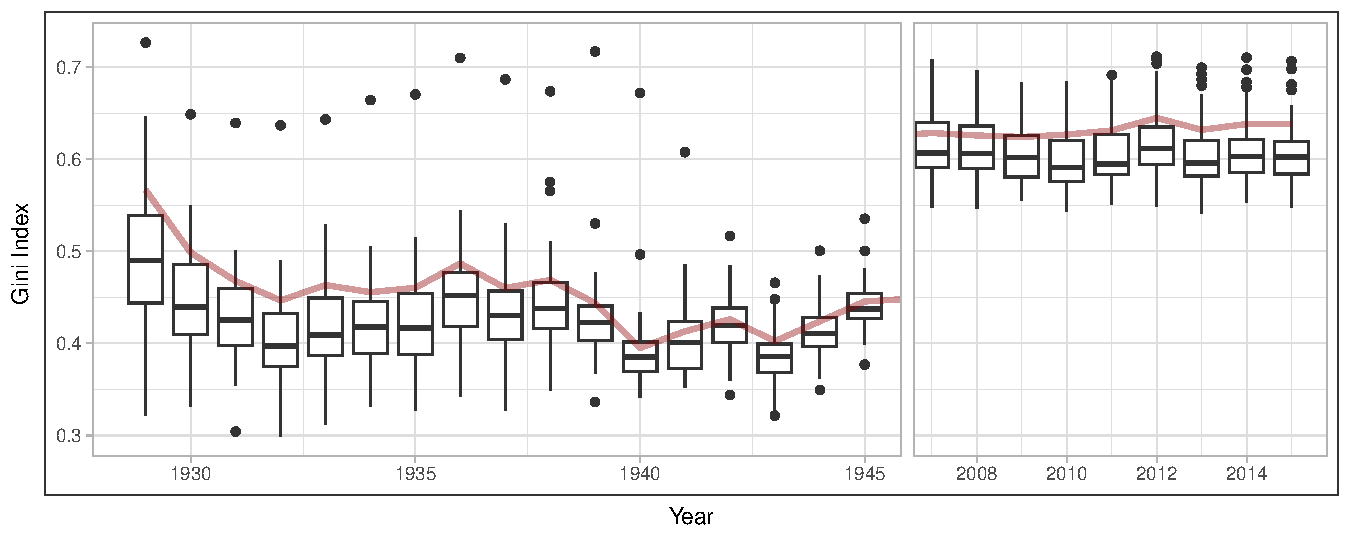
\includegraphics{Assignment_2_ETF5500_files/figure-latex/edaboxplot-1.pdf}
\caption{\label{fig:edaboxplot}Distribution of Gini Index over the year}
\end{figure}

Figure \ref{fig:edaboxplot} illustrates the distribution of the Gini Index over the years (boxplots), accompanied by a comparison to the U.S.'s average Gini Index (red line). Our plot reveals an apparent decreasing trend in Gini Index during the initial period from 1929 to 1945, while there is a sustained presence of relatively high Gini Index levels during the subsequent period.

The boxplot also provides insights into the distribution characteristics of each year. The distributions display a degree of symmetry, accompanied by a slight right-skewness as the mean is marginally larger than the median in certain years. We observe that during the Great Depression and WWII, the variance of the Gini Index experiences a significant reduction, while it remains rather stable across the GFC period.

\begin{figure}
\centering
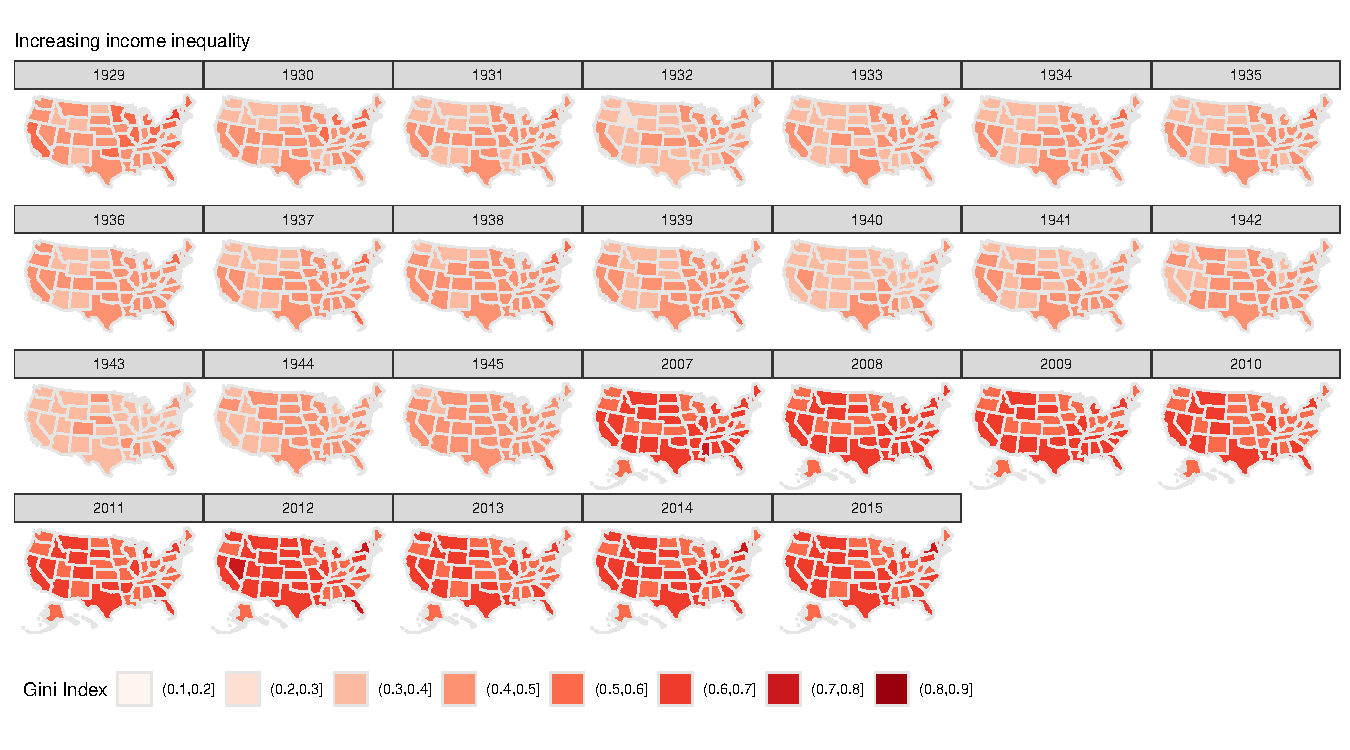
\includegraphics{Assignment_2_ETF5500_files/figure-latex/edamap-1.pdf}
\caption{\label{fig:edamap}Gini Index across U.S. states over time}
\end{figure}

Figure \ref{fig:edamap} visually illustrates the link between geographic location and income inequality across U.S. states. Initially, North-Eastern metropolitan states like New York, Massachusetts, Connecticut, Delaware, and Florida consistently displayed higher income inequality. Factors contributing to this include their status as economic hubs, especially in the finance sector, which offers high-paying jobs that contribute to income disparities. Additionally, the high cost of living exacerbates income gaps, particularly for lower-income individuals. Significant migration patterns involving both high and low-skilled workers further contribute to income disparities. In the subsequent period, income inequality variance among states reduced, coinciding with a nationwide worsening of income inequality. Nevertheless, New York and Florida remained notable for higher income inequality.

\newpage

\hypertarget{analysis}{%
\section{Analysis}\label{analysis}}

\hypertarget{assumptions}{%
\subsection{Assumptions}\label{assumptions}}

There are some assumptions that we employ when performing the analysis:

\begin{itemize}
\tightlist
\item
  We did not scale the data since the Gini Index already has consistent units of measurement.
\item
  The Euclidean method was used to calculate distances, capturing differences in Gini index values.
\item
  Hierarchical clustering was chosen due to the lack of prior data characteristics, allowing us to determine the appropriate cluster number during analysis.
\item
  The D2.Ward method was employed to minimise within-cluster variance and create compact clusters, with later assessments of its robustness and comparison with alternative methods.
\item
  We reduced dimensions to two in MDS for enhanced interpretability and visualization.
\end{itemize}

\newpage

\hypertarget{cluster-analysis}{%
\subsection{Cluster Analysis}\label{cluster-analysis}}

\hypertarget{period-1}{%
\subsubsection{Period 1}\label{period-1}}

\begin{figure}

{\centering 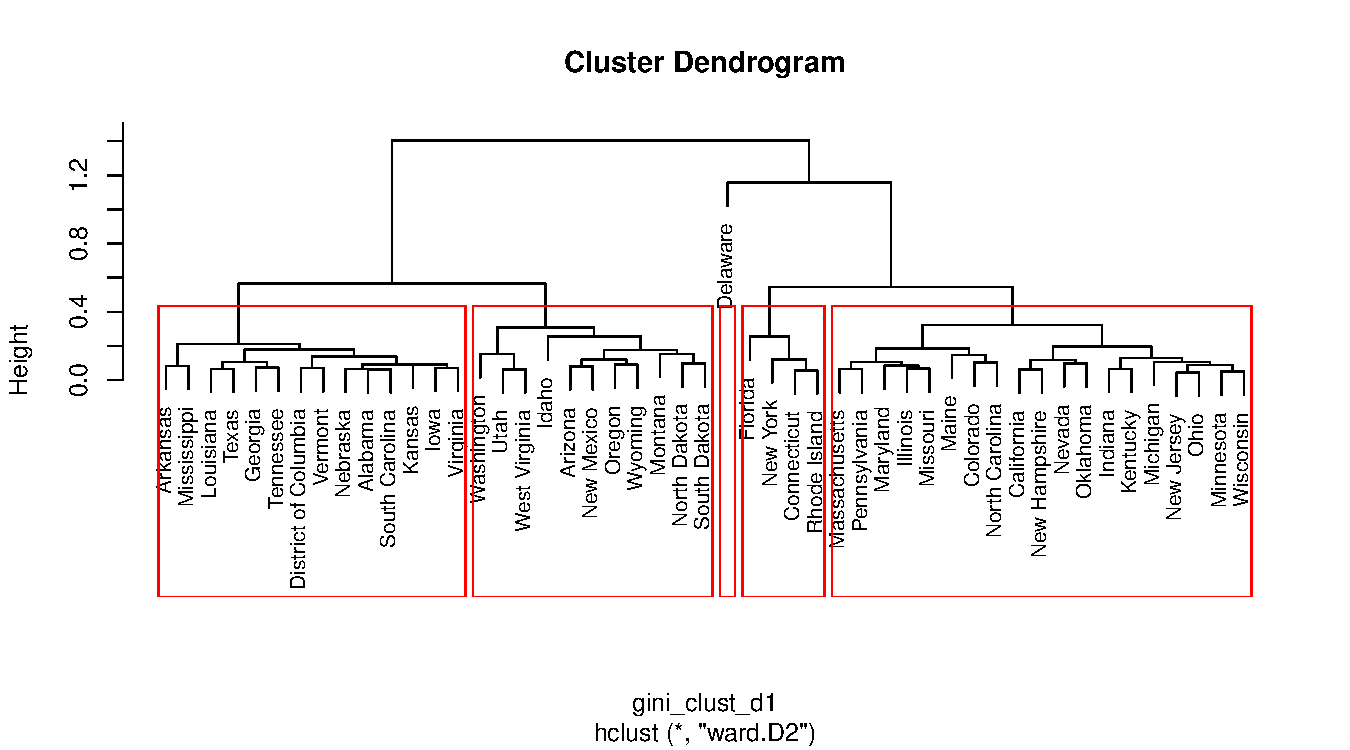
\includegraphics{Assignment_2_ETF5500_files/figure-latex/clust-1-dendrogram-1} 

}

\caption{Cluster Analysis of the 1st Period (1929 - 1945)}\label{fig:clust-1-dendrogram}
\end{figure}

From Figure \ref{fig:clust-1-dendrogram}, a stable solution with five clusters is observed within a tolerance range of 0.35 to 0.44. This configuration provides adequate grouping without sacrificing the detail within each cluster.

\begin{figure}
\centering
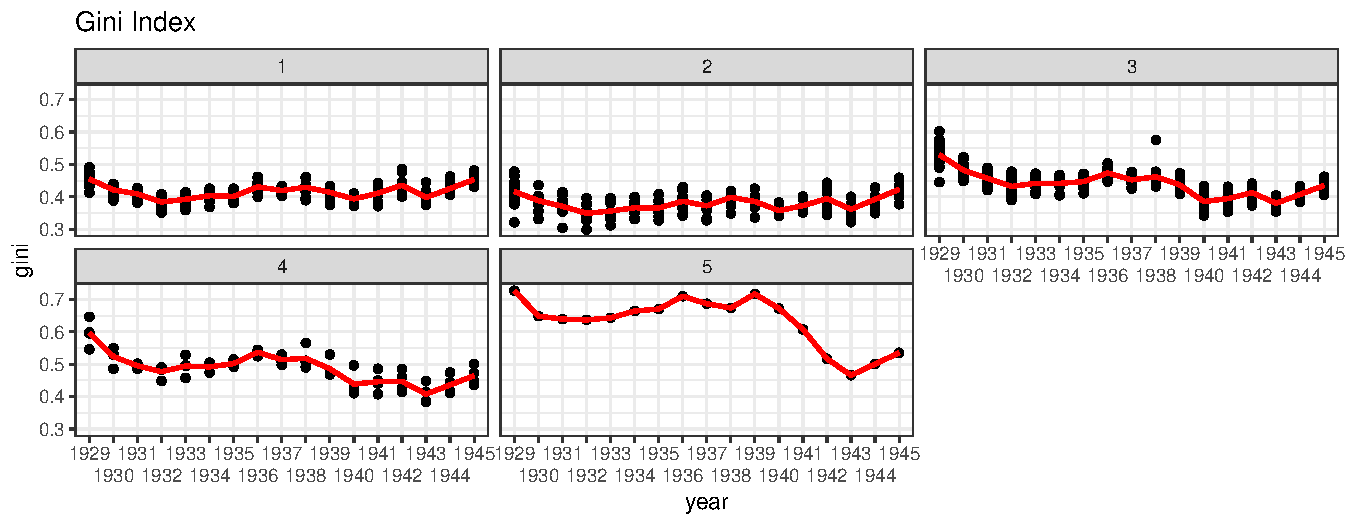
\includegraphics{Assignment_2_ETF5500_files/figure-latex/cluster-1-1.pdf}
\caption{\label{fig:cluster-1}Cluster Profiles for the 1st Period: Five-cluster Solution}
\end{figure}

Figure \ref{fig:cluster-1} visually illustrates the Gini Index for each cluster, along with an average line. Notably, during the Great Depression and WWII era, Delaware, part of cluster five, exhibited significantly higher inequality compared to the others, making it stand out.

Lastly, we assess the robustness of Ward's method against others by calculating the Adjusted Rand Index. Table \ref{tab:rand-1} in the appendix shows that Ward's method exhibits fairly strong robustness compared to alternative methods.

\newpage

\hypertarget{period-2}{%
\subsubsection{Period 2}\label{period-2}}

\begin{figure}

{\centering 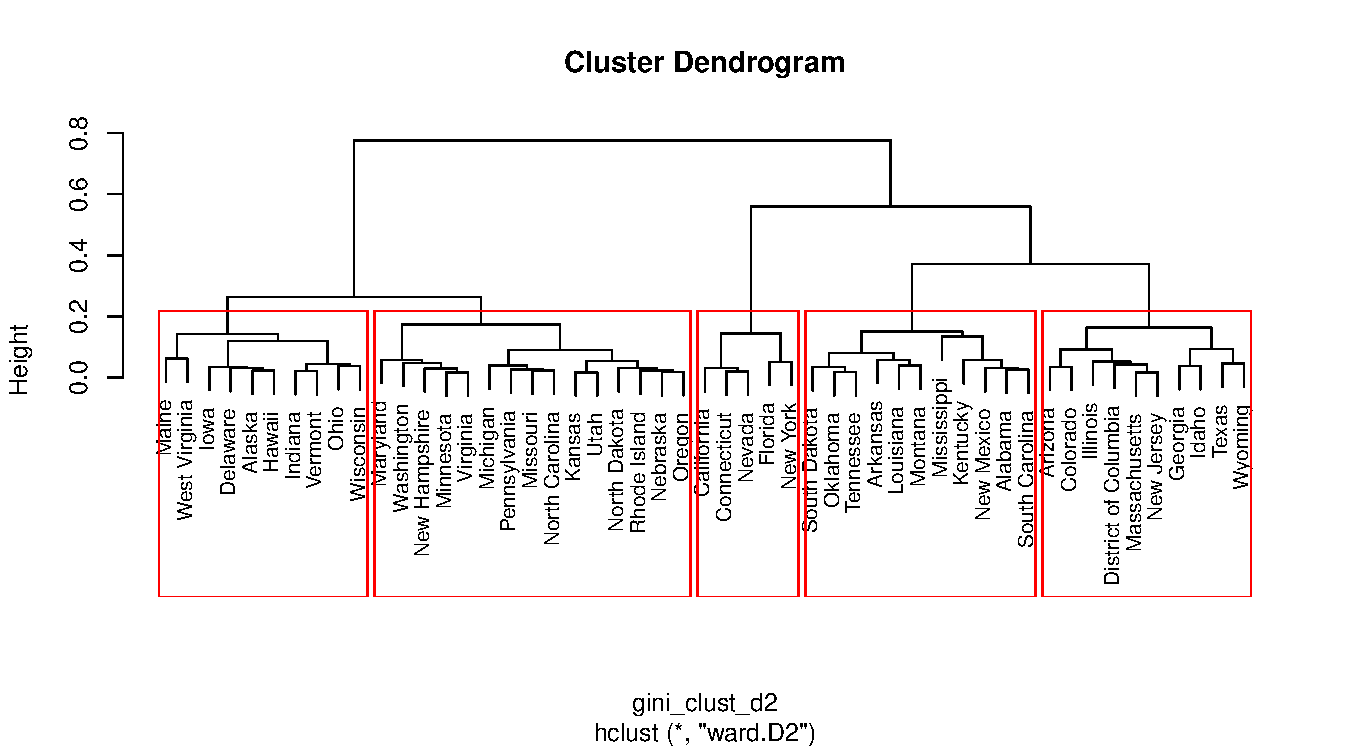
\includegraphics{Assignment_2_ETF5500_files/figure-latex/clust-2-dendrogram-1} 

}

\caption{Cluster Analysis of the 2nd Period (2007 - 2015)}\label{fig:clust-2-dendrogram}
\end{figure}

Figure \ref{fig:clust-2-dendrogram} also portrays a stable five-cluster solution within a tolerance range of 0.18 to 0.3.

\begin{figure}
\centering
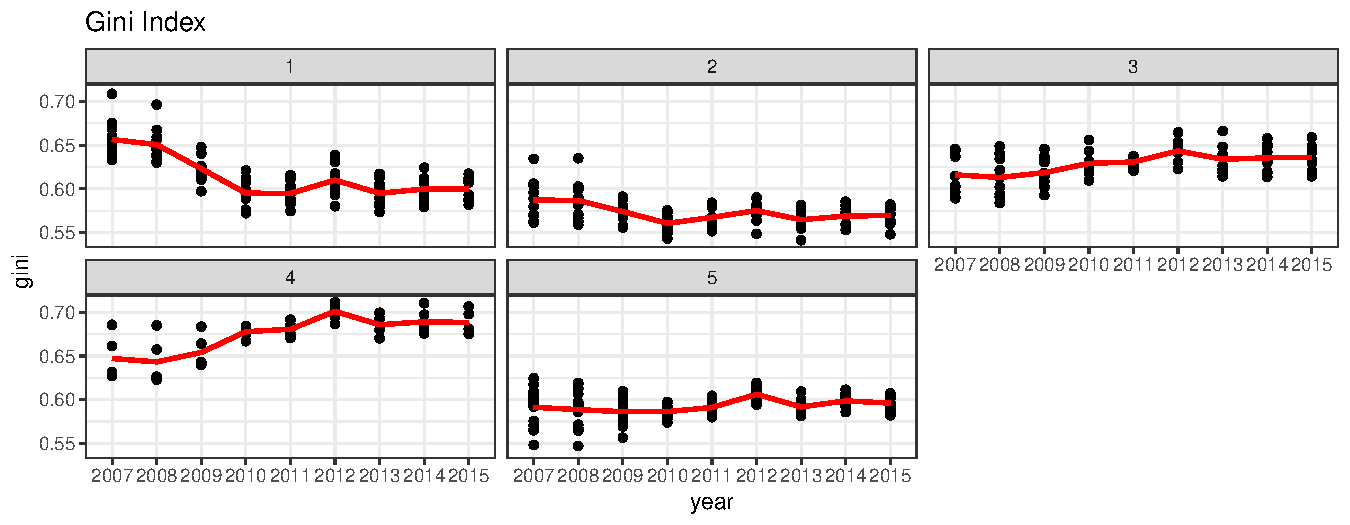
\includegraphics{Assignment_2_ETF5500_files/figure-latex/cluster-2-1.pdf}
\caption{\label{fig:cluster-2}Cluster Profiles for the 2nd Period: Five-cluster Solution}
\end{figure}

Figure \ref{fig:cluster-2} highlights cluster four as having the highest inequality. Table \ref{tab:gini2-clust4} provides a list of states within this cluster.

\begin{longtable}[]{@{}rrrrrrrrrrr@{}}
\caption{\label{tab:gini2-clust4}Cluster 4: states with the highest Gini Index}\tabularnewline
\toprule\noalign{}
Cluster & State & 2007 & 2008 & 2009 & 2010 & 2011 & 2012 & 2013 & 2014 & 2015 \\
\midrule\noalign{}
\endfirsthead
\toprule\noalign{}
Cluster & State & 2007 & 2008 & 2009 & 2010 & 2011 & 2012 & 2013 & 2014 & 2015 \\
\midrule\noalign{}
\endhead
\bottomrule\noalign{}
\endlastfoot
4 & California & 0.630 & 0.626 & 0.640 & 0.667 & 0.671 & 0.687 & 0.670 & 0.678 & 0.675 \\
4 & Connecticut & 0.627 & 0.624 & 0.640 & 0.675 & 0.675 & 0.695 & 0.680 & 0.684 & 0.681 \\
4 & Florida & 0.686 & 0.685 & 0.684 & 0.682 & 0.685 & 0.711 & 0.693 & 0.697 & 0.698 \\
4 & Nevada & 0.632 & 0.623 & 0.643 & 0.682 & 0.681 & 0.704 & 0.686 & 0.676 & 0.681 \\
4 & New York & 0.661 & 0.657 & 0.664 & 0.684 & 0.691 & 0.708 & 0.699 & 0.710 & 0.707 \\
\end{longtable}

Regarding the robustness analysis, as shown in Table \ref{tab:rand-2} in the Appendix, we can conclude that Ward's method is relatively robust compared to other methods.

\newpage

\hypertarget{multidimensional-scaling-mds}{%
\subsection{Multidimensional Scaling (MDS)}\label{multidimensional-scaling-mds}}

\hypertarget{period-1-1}{%
\subsubsection{Period 1}\label{period-1-1}}

\begin{figure}
\centering
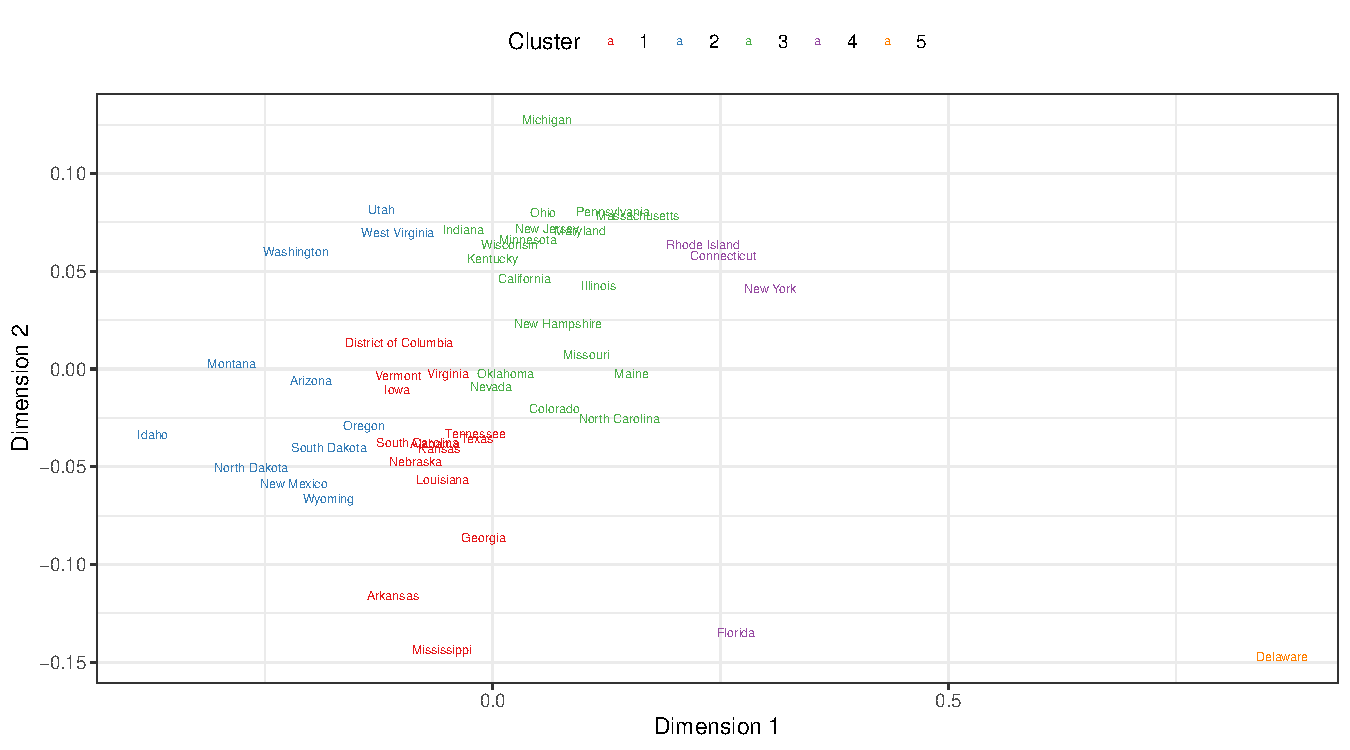
\includegraphics{Assignment_2_ETF5500_files/figure-latex/mds1-1.pdf}
\caption{\label{fig:mds1}MDS by U.S. state for the 1st period (1929 - 1945)}
\end{figure}

\begin{figure}
\centering
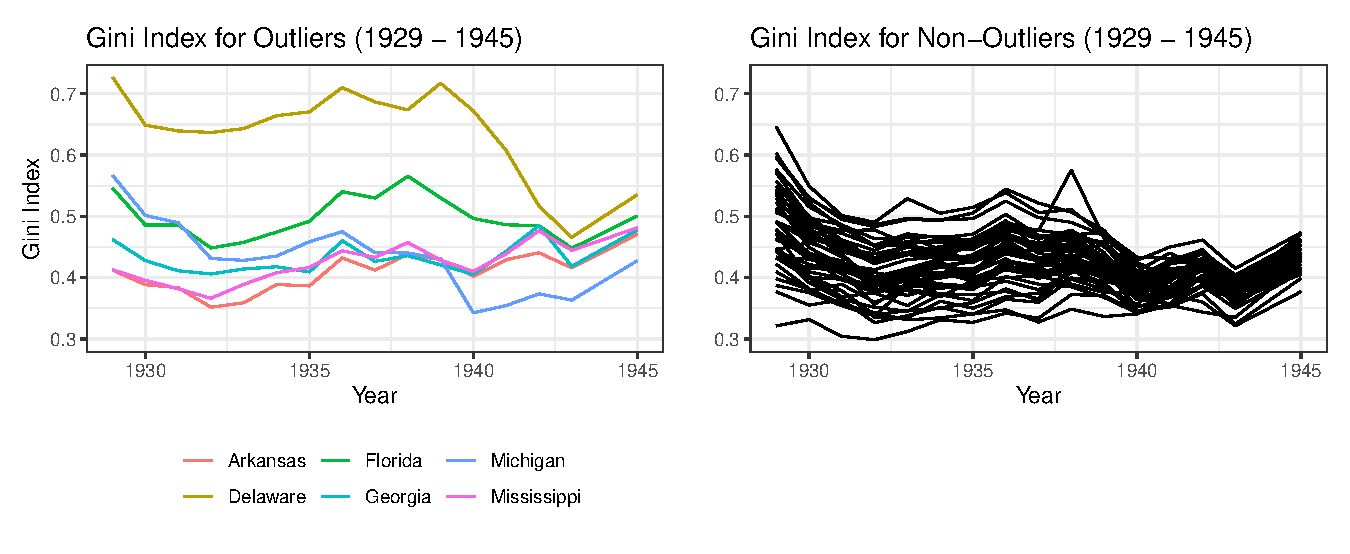
\includegraphics{Assignment_2_ETF5500_files/figure-latex/mds1-line-1.pdf}
\caption{\label{fig:mds1-line}Gini Index of the outlier states between 1929 and 1945}
\end{figure}

Figure \ref{fig:mds1} reveals that states cluster near the center of the plot on both axes, suggesting lower Gini indices during the Great Depression/WWII in comparison to states located further from the center.

\newpage

\hypertarget{period-2-1}{%
\subsubsection{Period 2}\label{period-2-1}}

\begin{figure}
\centering
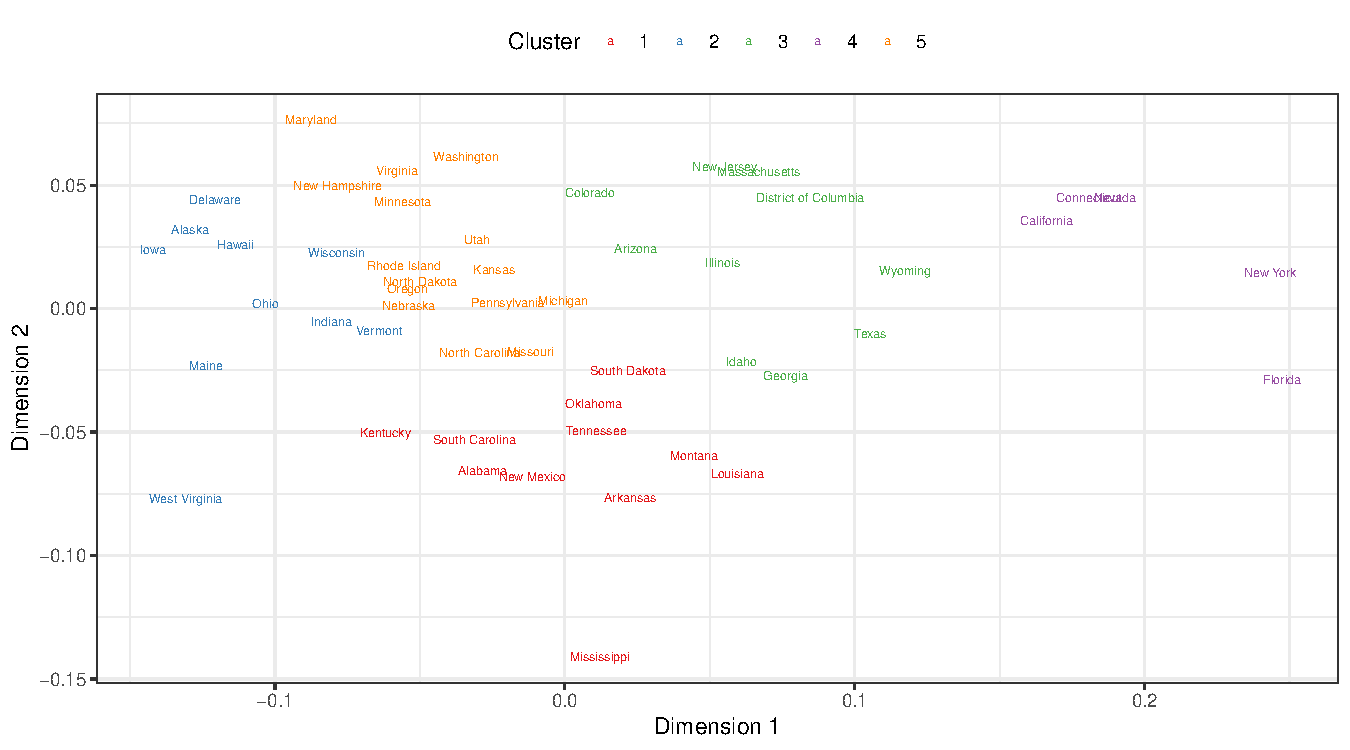
\includegraphics{Assignment_2_ETF5500_files/figure-latex/mds2-1.pdf}
\caption{\label{fig:mds2}MDS by U.S. state for the 2nd period (2007 - 2015)}
\end{figure}

\begin{figure}
\centering
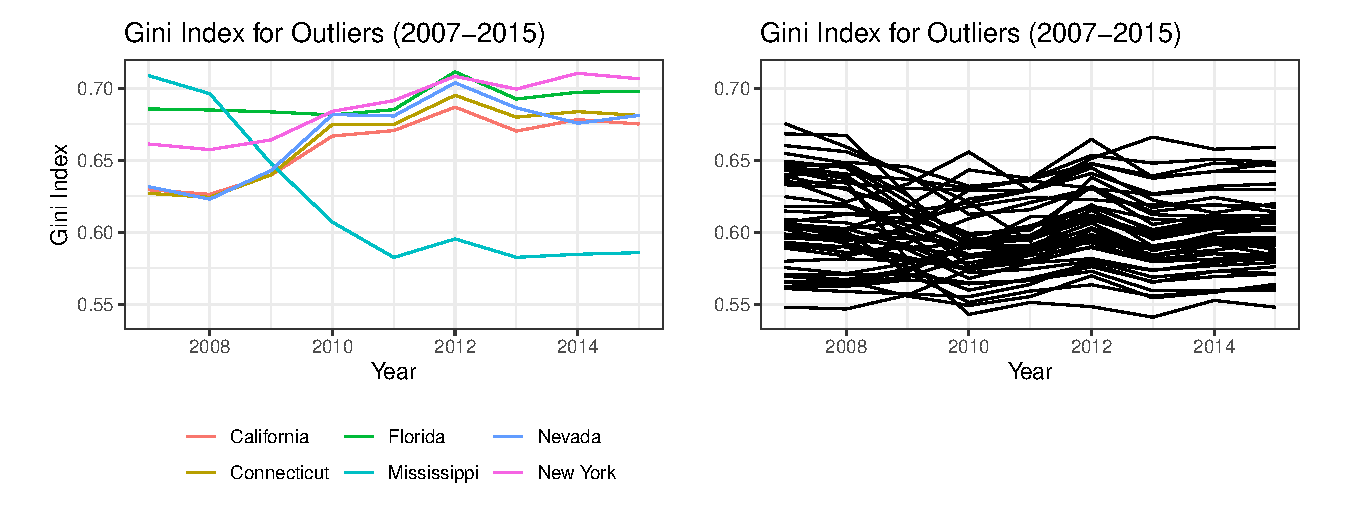
\includegraphics{Assignment_2_ETF5500_files/figure-latex/mds2-line-1.pdf}
\caption{\label{fig:mds2-line}Gini Index of the outlier states between 2007 and 2015}
\end{figure}

Figure \ref{fig:mds2} reveals increased state dispersion away from the origin, implying higher income inequality during the GFC compared to the Great Depression/WWII era. In particular, New York, Florida, and Mississippi are outliers, while California, Connecticut, and Nevada cluster near New York's position.

\newpage

\hypertarget{principal-component-analysis-pca}{%
\subsection{Principal Component Analysis (PCA)}\label{principal-component-analysis-pca}}

\hypertarget{period-1-2}{%
\subsubsection{Period 1}\label{period-1-2}}

\hypertarget{kaisers-rule}{%
\paragraph{Kaiser's rule}\label{kaisers-rule}}

\begingroup\fontsize{8}{10}\selectfont

\begin{longtable}[t]{lcccccccccc}
\caption{\label{tab:summary-period1}Importance of components - 1st Period}\\
\toprule
  & PC1 & PC2 & PC3 & PC4 & PC5 & PC6 & PC7 & PC8 & PC9 & PC10\\
\midrule
Standard deviation & 3.5896 & 1.6142 & 0.7831 & 0.5699 & 0.3549 & 0.3501 & 0.2993 & 0.2405 & 0.2173 & 0.2005\\
Proportion of Variance & 0.7580 & 0.1533 & 0.0361 & 0.0191 & 0.0074 & 0.0072 & 0.0053 & 0.0034 & 0.0028 & 0.0024\\
Cumulative Proportion & 0.7580 & 0.9112 & 0.9473 & 0.9664 & 0.9738 & 0.9810 & 0.9863 & 0.9897 & 0.9925 & 0.9948\\
\bottomrule
\end{longtable}
\endgroup{}

According to Table \ref{tab:summary-period1}, following Kaiser's rule, we select 2 principal components (PCs) since both the variance and standard deviation are greater than 1, and the cumulative proportion of variance is 91.12\%.

\hypertarget{distance-bi-plot}{%
\paragraph{\texorpdfstring{Distance bi-plot \(\\\)}{Distance bi-plot \textbackslash\textbackslash{}}}\label{distance-bi-plot}}

\begin{figure}

{\centering 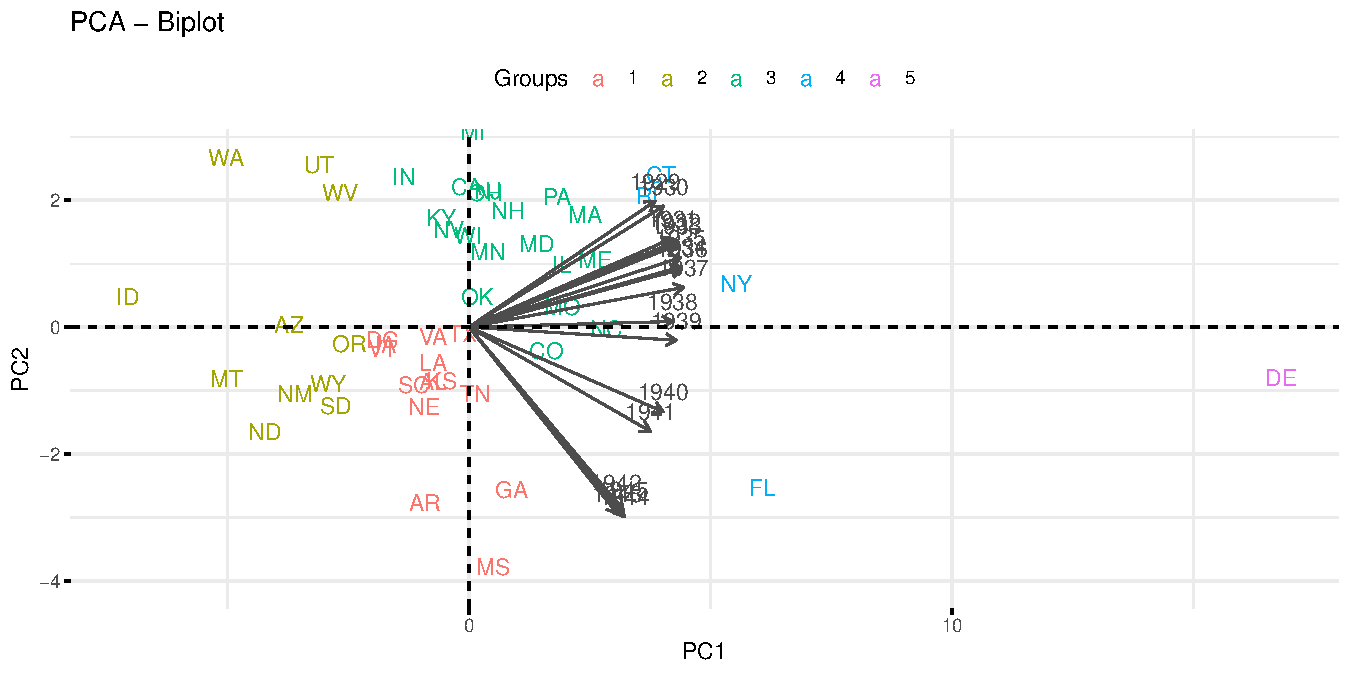
\includegraphics{Assignment_2_ETF5500_files/figure-latex/dbiplot-period1-1} 

}

\caption{Distance Biplot - PCA of the 1st period}\label{fig:dbiplot-period1}
\end{figure}

\(\\\)
In Figure \ref{fig:dbiplot-period1}, the years 1937-1939 closely align with PC1, coinciding with the start of WWII. Due to increased military spending, \textcite{pellsromer2023} shows a 9\% GDP growth from 1933 to 1937 whilst \textcite{waiwood2013} notes a 10\% drop in unemployment rates. Therefore, PC1 characterises higher GDP and lower unemployment, representing the US's recovery from the Great Depression.

Delaware's (DE) high PC1 values, indicating a strong GDP and employment rate at the start of WWII, are linked to its key role in gunpowder manufacturing and shipyards (\textcite{rowe1980}). However, this led to increased income inequality as top industry leaders prospered. The influx of migrants for jobs during WWII further widened income disparities due to limited opportunities and lower wages for these migrants. As a result, Delaware had the highest Gini index, with its top earners making two to three times more than their counterparts in other states (\textcite{schmitz1983}; Figure \ref{fig:mds1-line})

Meanwhile, Idaho (ID) has low PC1 values, indicating low average real GDP and employment rates at the onset of WWII. According to \textcite{BID}, this is unsurprising given Idaho's heavy reliance on agriculture and limited industrial capacity in the 1930s. This economic dependence on agriculture, coupled with falling food prices and reduced agricultural income during the Great Depression, likely worsened its income inequality.

Figure \ref{fig:dbiplot-period1} associates high PC2 values with GDP decline and unemployment surge during the Great Depression (1929-1933), while lower PC2 values correspond to economic growth and job increase in WWII's later years (1942-1945). As noted by \textcite{duignan2018}, US' industrial production fell by nearly 47\% between 1929 and 1933, leading to a 30\% GDP reduction and unemployment rates peaking at over 20\%. In contrast, extensive military production drove up US' real GDP by 72\% from 1940-1945, with unemployment rates falling from 9.5\% in 1940 to below 2\% from 1943-1945 (\textcite{fishback2019}).

Mississippi's (MS) low PC2 values reflect the significant economic benefits reaped during WWII. As per \textcite{SJ17}, income per capita increased substantially by 11\%, and urban employment opportunities grew as the farm population decreased by 26\%, with many joining the military.

States such as Tennessee, Alabama, Kansas, Nebraska, Louisiana, and Arkansas experienced lower PC2 values during the 1929-1933 period. These Southern and Midwestern states faced economic difficulties due to widespread poverty and heavy reliance on farming (\textcite{davis1978south}). Roosevelt's New Deal policies played a pivotal role in revitalising agriculture, stimulating economic growth and creating jobs (\textcite{nourse1936fundamental}), which aided these regions in recovering from the Great Depression and stabilising income inequality.

\hypertarget{correlation-bi-plot}{%
\paragraph{Correlation bi-plot}\label{correlation-bi-plot}}

\(\\\)

\begin{figure}

{\centering 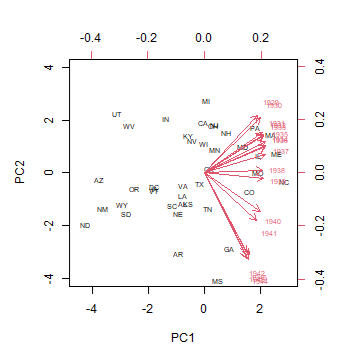
\includegraphics[width=0.5\linewidth]{../image/cbiplot-period1} 

}

\caption{Correlation Biplot - PCA of the 1st period}\label{fig:cbiplot-period1}
\end{figure}

Based on Figure \ref{fig:cbiplot-period1}, some years show little correlation. For example, the years 1929 and 1941, as well as 1934 and 1942, have angles close to 90 degrees between them. This lack of correlation is because the Great Depression lasted from 1929 to 1939, while WWII occurred from 1939 to 1945. In contrast, 1929 and 1945 have a strong negative correlation, with an angle close to 180 degrees, as the former marks the start of the Great Depression and the latter the end of WWII. These correlations reflect the distinct historical contexts and economic conditions of these years.

\newpage

\hypertarget{period-2-2}{%
\subsubsection{Period 2}\label{period-2-2}}

\hypertarget{kaisers-rule-1}{%
\paragraph{Kaiser's rule}\label{kaisers-rule-1}}

\begingroup\fontsize{8}{10}\selectfont

\begin{longtable}[t]{lrrrrrrrrr}
\caption{\label{tab:summary-period2}Importance of components - 2nd Period}\\
\toprule
  & PC1 & PC2 & PC3 & PC4 & PC5 & PC6 & PC7 & PC8 & PC9\\
\midrule
Standard deviation & 2.6752 & 1.3084 & 0.2128 & 0.1829 & 0.1613 & 0.1121 & 0.0835 & 0.0742 & 0.0401\\
Proportion of Variance & 0.7952 & 0.1902 & 0.0050 & 0.0037 & 0.0029 & 0.0014 & 0.0008 & 0.0006 & 0.0002\\
Cumulative Proportion & 0.7952 & 0.9854 & 0.9904 & 0.9942 & 0.9970 & 0.9984 & 0.9992 & 0.9998 & 1.0000\\
\bottomrule
\end{longtable}
\endgroup{}

According to Table \ref{tab:summary-period2}, we choose two PCs based on Kaiser's rule, as both the variance and standard deviation are greater than 1, and the cumulative proportion of explained variance is 98.54\%.

\hypertarget{distance-bi-plot-1}{%
\paragraph{\texorpdfstring{Distance bi-plot \(\\\)}{Distance bi-plot \textbackslash\textbackslash{}}}\label{distance-bi-plot-1}}

\begin{figure}

{\centering 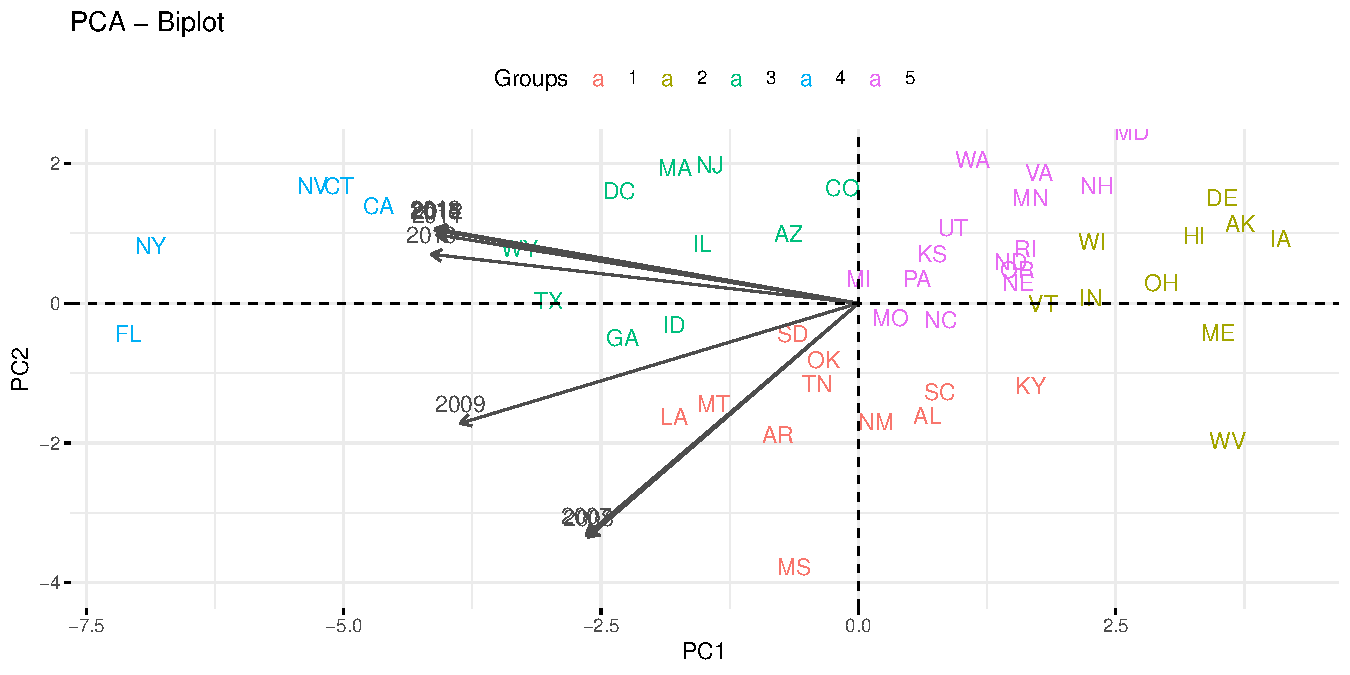
\includegraphics{Assignment_2_ETF5500_files/figure-latex/dbiplot-period2-1} 

}

\caption{Distance Biplot - PCA of the 2nd period}\label{fig:dbiplot-period2}
\end{figure}

\(\\\)
Figure \ref{fig:dbiplot-period2} displays a distance biplot, highlighting the association between PC2 and the GFC, while PC1 corresponds to the `recovery period.' According to data from \textcite{worldbank2023}, the U.S. experienced a GDP decline during the GFC, reflecting the economic downturn characterized by business struggles, reduced consumer spending, and shrinking investments. Subsequent GDP growth indicates a shift away from recession.

The employment rate in the U.S. significantly dropped in the early 2007 period and began a gradual increase (\textcite{worldbank2023unemployment}). The GFC's global impact exacerbated the situation, with decreased global demand for U.S. exports contributing to rising unemployment. Additionally, a decline in inflation during 2007-2008 (\textcite{worldbank2023inflation}) can be attributed to the GFC, as economic contraction led to reduced demand, business challenges, and job losses.

The biplot highlights significant income inequality in states like Florida, New York, and Nevada, where affluent individuals tend to cluster in urban areas such as Miami, New York City, and Las Vegas. This concentration of wealth resulted in high Gini Index values during and after the GFC. In Florida and New York, the richest 1\% of households accounted for a substantial 61\% of the adjusted gross income, as indicated by \textcite{cbpp2012}.

California and Texas were also heavily affected by the GFC, primarily due to their reliance on manufacturing and construction, as reported by \textcite{usbls2010}. In contrast, Delaware showed a declining Gini Index during both the GFC and the recovery period. This trend might be attributed to its progressive tax rates, potentially leading to wealthier households migrating out, as suggested by \textcite{vuoccolo2018}.

\hypertarget{correlation-bi-plot-1}{%
\paragraph{Correlation bi-plot}\label{correlation-bi-plot-1}}

\(\\\)

\begin{figure}

{\centering 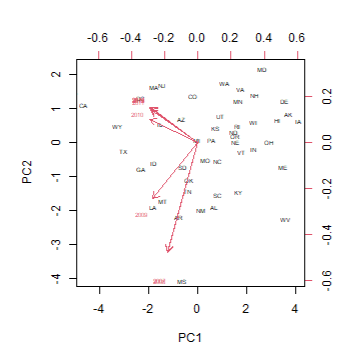
\includegraphics[width=0.5\linewidth]{../image/cbiplot-period2} 

}

\caption{Correlation Biplot - PCA of the 2nd period}\label{fig:cbiplot-period2}
\end{figure}

In Figure \ref{fig:cbiplot-period2}, strong positive correlations are observed for specific years, notably 2007 and 2008, reflecting the impact of the GFC. 2011-2015 exhibit similar patterns, likely associated with economic recovery. However, 2009 and 2012 appear uncorrelated, indicating the U.S. transition from recession to growth. Notably, there are no significant negative correlations among the years.

\newpage

\hypertarget{limitations}{%
\section{Limitations}\label{limitations}}

Several limitations that surfaced during our analysis include:

\textbf{Cluster Analysis}

\begin{itemize}
\tightlist
\item
  Optimal cluster number determination can be subjective and challenging due to methodological variations.
\item
  Outliers and data noise can impact cluster quality and sensitivity.
\end{itemize}

\textbf{Multidimensional Scaling (MDS)}

\begin{itemize}
\tightlist
\item
  MDS reveals data similarities/differences but does not offer causal explanations for state-specific income inequality patterns.
\item
  MDS may not capture all nuances in the original data, potentially leading to information loss. To address this, we calculated Goodness of Fit (GOF) values, which were approximately 0.934 in period 1 and 0.985 in period 2 (see Appendix's Table \ref{tab:rand-1}). These indicate varying degrees of alignment between MDS plots and the original data, with period 2 showing a higher degree of accuracy.
\end{itemize}

\textbf{Principal Component Analysis}

Interpreting PCA results can be challenging without sufficient domain knowledge. To address this, we conducted extensive research on relevant historical events to provide context and support our interpretation of the PCA findings.

\newpage

\hypertarget{conclusion}{%
\section{Conclusion}\label{conclusion}}

Our analysis of income inequality during the Great Depression, WWII, and the GFC revealed significant findings:

\textbf{The Great Depression/WWII}

\begin{itemize}
\tightlist
\item
  A five-cluster approach effectively groups states for detailed analysis.
\item
  States closer to the center in our MDS analysis show lower income inequality during these periods.
\item
  PC1 reflects higher GDP and lower unemployment, indicating recovery from the Great Depression.
\item
  PC2 strongly correlates with economic conditions during these events.
\end{itemize}

\textbf{The Global Financial Crisis (GFC)}

\begin{itemize}
\tightlist
\item
  A five-cluster solution is again useful for meaningful groupings.\\
\item
  States shifted away from the center in our MDS analysis, indicating increased income inequality overall compared to the previous era.
\item
  PC1 aligns with the GFC recovery period (2009--2015), while PC2 relates to the GFC itself (2007 - 2008), reflecting changes in US' GDP.
\end{itemize}

In summary, our analysis provided valuable insights into income inequality during critical historical events. To enhance our understanding, we recommend incorporating Factor Models and additional economic indicators. This will help us better interpret the complex economic dynamics shaped by these significant events.

\newpage

\hypertarget{appendix}{%
\section{Appendix}\label{appendix}}

\hypertarget{appendix-1-analysis}{%
\subsection{Appendix 1: Analysis}\label{appendix-1-analysis}}

\begingroup\fontsize{8}{10}\selectfont

\begin{longtable}[t]{cccccc}
\caption{\label{tab:unnamed-chunk-6}Summary by Year}\\
\toprule
Year & Min & 1st Qu. & Median & 3rd Qu. & Max\\
\midrule
1929 & 0.321 & 0.444 & 0.490 & 0.539 & 0.727\\
1930 & 0.331 & 0.409 & 0.440 & 0.486 & 0.649\\
1931 & 0.304 & 0.397 & 0.425 & 0.459 & 0.639\\
1932 & 0.299 & 0.375 & 0.397 & 0.433 & 0.637\\
1933 & 0.312 & 0.387 & 0.409 & 0.449 & 0.643\\
\addlinespace
1934 & 0.331 & 0.389 & 0.418 & 0.446 & 0.664\\
1935 & 0.327 & 0.388 & 0.417 & 0.454 & 0.670\\
1936 & 0.342 & 0.419 & 0.452 & 0.477 & 0.710\\
1937 & 0.327 & 0.404 & 0.430 & 0.457 & 0.687\\
1938 & 0.349 & 0.416 & 0.438 & 0.467 & 0.674\\
\addlinespace
1939 & 0.336 & 0.403 & 0.423 & 0.441 & 0.717\\
1940 & 0.341 & 0.370 & 0.385 & 0.402 & 0.672\\
1941 & 0.352 & 0.372 & 0.401 & 0.424 & 0.608\\
1942 & 0.344 & 0.401 & 0.420 & 0.438 & 0.517\\
1943 & 0.322 & 0.368 & 0.386 & 0.399 & 0.466\\
\addlinespace
1944 & 0.349 & 0.397 & 0.411 & 0.428 & 0.501\\
1945 & 0.377 & 0.427 & 0.438 & 0.455 & 0.535\\
2007 & 0.548 & 0.591 & 0.607 & 0.640 & 0.709\\
2008 & 0.547 & 0.590 & 0.607 & 0.636 & 0.696\\
2009 & 0.556 & 0.581 & 0.602 & 0.626 & 0.684\\
\addlinespace
2010 & 0.543 & 0.576 & 0.591 & 0.621 & 0.684\\
2011 & 0.551 & 0.583 & 0.595 & 0.627 & 0.691\\
2012 & 0.548 & 0.594 & 0.612 & 0.635 & 0.711\\
2013 & 0.541 & 0.582 & 0.596 & 0.621 & 0.699\\
2014 & 0.553 & 0.585 & 0.603 & 0.622 & 0.710\\
\addlinespace
2015 & 0.548 & 0.584 & 0.603 & 0.619 & 0.707\\
\bottomrule
\end{longtable}
\endgroup{}

\hypertarget{cluster-analysis-1}{%
\subsubsection{Cluster Analysis}\label{cluster-analysis-1}}

\begingroup\fontsize{10}{12}\selectfont

\begin{longtable}[t]{lrrr}
\caption{\label{tab:rand-1}Evaluating the robustness of the model - 1st Period}\\
\toprule
  & Average Linkage & Centroid & Complete Linkage\\
\midrule
Ward's Method & 0.715 & 0.203 & 1\\
\bottomrule
\end{longtable}
\endgroup{}

\begingroup\fontsize{10}{12}\selectfont

\begin{longtable}[t]{lrrr}
\caption{\label{tab:rand-2}Evaluating the robustness of the model - 2st Period}\\
\toprule
  & Average Linkage & Centroid & Complete Linkage\\
\midrule
Ward's Method & 0.63 & 0.198 & 0.395\\
\bottomrule
\end{longtable}
\endgroup{}

\hypertarget{mds}{%
\subsubsection{MDS}\label{mds}}

\begin{longtable}[]{@{}rrr@{}}
\caption{\label{tab:mds-gof}MDS Goodness of Fit}\tabularnewline
\toprule\noalign{}
Period & GOF1 & GOF2 \\
\midrule\noalign{}
\endfirsthead
\toprule\noalign{}
Period & GOF1 & GOF2 \\
\midrule\noalign{}
\endhead
\bottomrule\noalign{}
\endlastfoot
1st & 0.9340 & 0.9340 \\
2nd & 0.9855 & 0.9855 \\
\end{longtable}

\hypertarget{pca}{%
\subsubsection{PCA}\label{pca}}

\textbf{Scree plot}

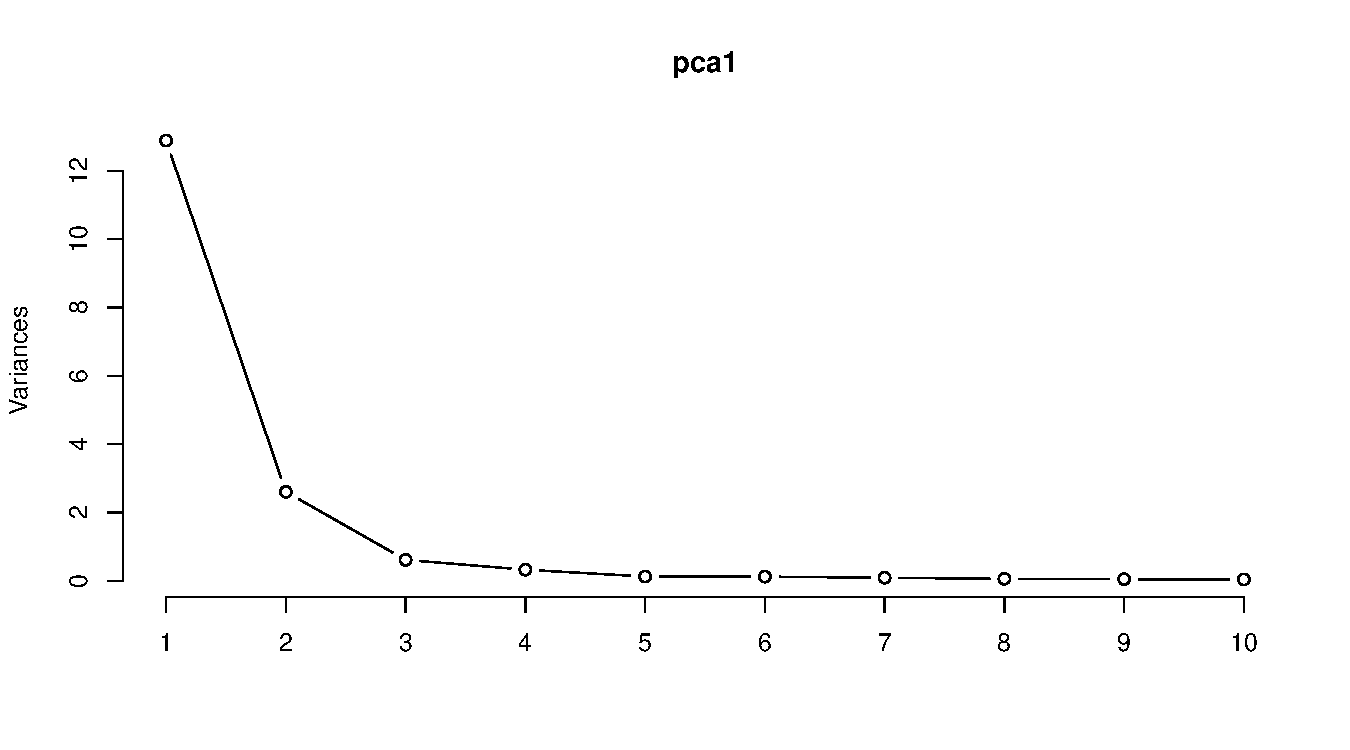
\includegraphics[width=0.49\linewidth]{Assignment_2_ETF5500_files/figure-latex/screeplot-period1, figures-side-1} 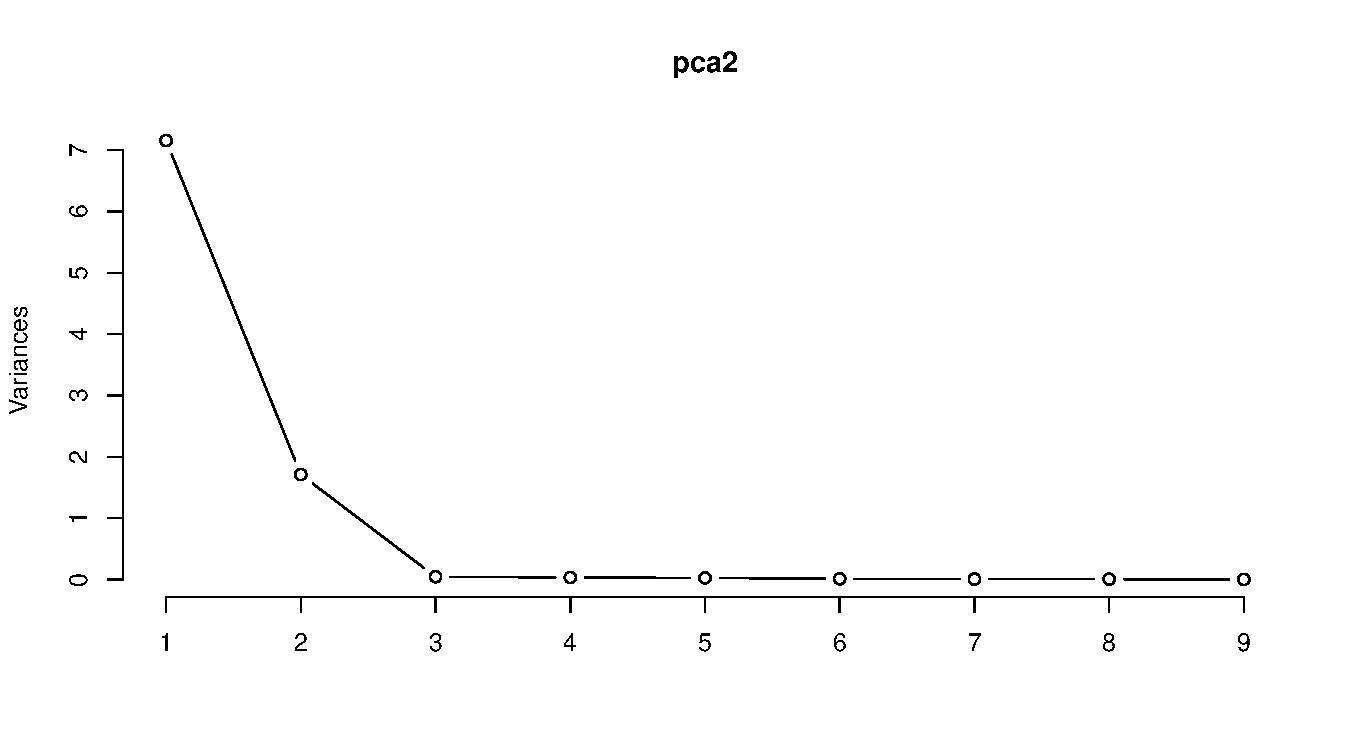
\includegraphics[width=0.49\linewidth]{Assignment_2_ETF5500_files/figure-latex/screeplot-period1, figures-side-2}

The Scree plot of both periods show that the ``elbow point'' is in the third point. These three point is sufficient for dimensionality reduction.

\textbf{Weights of the first two PCs}

\textbf{1st Period}

\begingroup\fontsize{10}{12}\selectfont

\begin{longtable}[t]{lrr}
\caption{\label{tab:weights-period1}Weights of the first two PCs - 1st Period}\\
\toprule
  & PC1 & PC2\\
\midrule
1929 & 0.2350 & 0.2690\\
1930 & 0.2459 & 0.2586\\
1931 & 0.2571 & 0.1897\\
1932 & 0.2604 & 0.1821\\
1933 & 0.2617 & 0.1744\\
\addlinespace
1934 & 0.2681 & 0.1289\\
1935 & 0.2674 & 0.1489\\
1936 & 0.2688 & 0.1243\\
1937 & 0.2711 & 0.0848\\
1938 & 0.2570 & 0.0118\\
\addlinespace
1939 & 0.2617 & -0.0283\\
1940 & 0.2452 & -0.1810\\
1941 & 0.2292 & -0.2230\\
1942 & 0.1856 & -0.3754\\
1943 & 0.1871 & -0.3985\\
\addlinespace
1944 & 0.1960 & -0.4054\\
1945 & 0.1944 & -0.3902\\
\bottomrule
\end{longtable}
\endgroup{}

Based on Table \ref{tab:weights-period1}, in 1937, PC1's high weight suggests a strong link between that year and PC1. PC2's high weight for 1929 indicates a strong connection between 1929 and PC2. The Great Depression, starting in 1929, had a significant impact on 1937, likely due to enduring economic hardships, including high unemployment and income disparities. From 1939 to 1945, PC2 consistently had negative values, implying reduced income inequality in other years, likely driven by increased job opportunities and higher incomes during WWII (1939-1945).

\textbf{2nd Period}\\
\begingroup\fontsize{10}{12}\selectfont

\begin{longtable}[t]{lrr}
\caption{\label{tab:weights-period2}Weights of the first two PCs - 2nd Period}\\
\toprule
  & PC1 & PC2\\
\midrule
2007 & -0.2318 & -0.5958\\
2008 & -0.2299 & -0.6004\\
2009 & -0.3391 & -0.3082\\
2010 & -0.3638 & 0.1260\\
2011 & -0.3589 & 0.1762\\
\addlinespace
2012 & -0.3586 & 0.1868\\
2013 & -0.3603 & 0.1915\\
2014 & -0.3594 & 0.1895\\
2015 & -0.3601 & 0.1874\\
\bottomrule
\end{longtable}
\endgroup{}

Based on Table \ref{tab:weights-period2}, negative PC1 values imply decreased income inequality, particularly during the GFC, while positive PC1 values highlight the significant impact of the crisis on income disparities. The shift from negative PC2 values (2007-2009) to positive (2010-2015) suggests changing income inequality patterns, possibly influenced by the Great Recession and subsequent economic factors.

\newpage

\hypertarget{appendix-2-code}{%
\subsection{Appendix 2: Code}\label{appendix-2-code}}

\textbf{Data Cleaning \& Preliminary Analysis}\\
\tiny  

\begin{Shaded}
\begin{Highlighting}[]
\CommentTok{\# DATA CLEANING {-}{-}{-}{-}{-}{-}{-}{-}{-}{-}{-}{-}{-}{-}{-}{-}{-}{-}{-}{-}{-}{-}{-}{-}{-}{-}{-}{-}{-}{-}{-}{-}{-}{-}{-}{-}}
\CommentTok{\# Get Data}
\NormalTok{gd }\OtherTok{\textless{}{-}} \FunctionTok{read\_csv}\NormalTok{(here}\SpecialCharTok{::}\FunctionTok{here}\NormalTok{(}\StringTok{"data/Inequality\_GD.csv"}\NormalTok{))}
\NormalTok{gr }\OtherTok{\textless{}{-}} \FunctionTok{read\_csv}\NormalTok{(here}\SpecialCharTok{::}\FunctionTok{here}\NormalTok{(}\StringTok{"data/Inequality\_GR.csv"}\NormalTok{))}

\CommentTok{\# Bind two raw datasets}
\NormalTok{gini }\OtherTok{\textless{}{-}} \FunctionTok{rbind}\NormalTok{(}
\NormalTok{  gd }\SpecialCharTok{\%\textgreater{}\%}\NormalTok{  dplyr}\SpecialCharTok{::}\FunctionTok{select}\NormalTok{(}\SpecialCharTok{{-}}\StringTok{"...1"}\NormalTok{) }\SpecialCharTok{\%\textgreater{}\%} 
    \FunctionTok{pivot\_longer}\NormalTok{(}\SpecialCharTok{{-}}\NormalTok{State, }\AttributeTok{names\_to =} \StringTok{"year"}\NormalTok{, }\AttributeTok{values\_to =} \StringTok{"gini"}\NormalTok{),}
\NormalTok{  gr }\SpecialCharTok{\%\textgreater{}\%}\NormalTok{ dplyr}\SpecialCharTok{::}\FunctionTok{select}\NormalTok{(}\SpecialCharTok{{-}}\StringTok{"...1"}\NormalTok{)}\SpecialCharTok{\%\textgreater{}\%} 
    \FunctionTok{pivot\_longer}\NormalTok{(}\SpecialCharTok{{-}}\NormalTok{State, }\AttributeTok{names\_to =} \StringTok{"year"}\NormalTok{, }\AttributeTok{values\_to =} \StringTok{"gini"}\NormalTok{)  }
\NormalTok{) }\SpecialCharTok{\%\textgreater{}\%} 
  \FunctionTok{rename}\NormalTok{(}\StringTok{"state\_name"} \OtherTok{=} \StringTok{"State"}\NormalTok{) }\SpecialCharTok{\%\textgreater{}\%} 
  \FunctionTok{mutate}\NormalTok{(}\AttributeTok{year =} \FunctionTok{as.numeric}\NormalTok{(year))}

\CommentTok{\# Add state abbreviation}
\NormalTok{state }\OtherTok{\textless{}{-}} \FunctionTok{tibble}\NormalTok{(}\AttributeTok{state\_name =} \FunctionTok{c}\NormalTok{(}\FunctionTok{unique}\NormalTok{(gini}\SpecialCharTok{$}\NormalTok{state\_name)))}
\NormalTok{state\_abb }\OtherTok{\textless{}{-}} \FunctionTok{data.frame}\NormalTok{(}\AttributeTok{state\_name =}\NormalTok{ state.name, }\AttributeTok{state =}\NormalTok{ state.abb)}
\NormalTok{state }\OtherTok{\textless{}{-}} \FunctionTok{left\_join}\NormalTok{(state, state\_abb, }\AttributeTok{by =} \FunctionTok{c}\NormalTok{(}\StringTok{"state\_name"} \OtherTok{=} \StringTok{"state\_name"}\NormalTok{)) }
\NormalTok{state }\OtherTok{\textless{}{-}}\NormalTok{ state }\SpecialCharTok{\%\textgreater{}\%} 
  \FunctionTok{mutate}\NormalTok{(}\AttributeTok{state =} \FunctionTok{case\_when}\NormalTok{(}
\NormalTok{    state\_name }\SpecialCharTok{==} \StringTok{"United States"} \SpecialCharTok{\textasciitilde{}} \StringTok{"US"}\NormalTok{,}
\NormalTok{    state\_name }\SpecialCharTok{==} \StringTok{"District of Columbia"} \SpecialCharTok{\textasciitilde{}} \StringTok{"DC"}\NormalTok{,}
    \ConstantTok{TRUE} \SpecialCharTok{\textasciitilde{}}\NormalTok{ state))}
\NormalTok{gini }\OtherTok{\textless{}{-}} \FunctionTok{left\_join}\NormalTok{(gini, state, }\AttributeTok{by =} \FunctionTok{c}\NormalTok{(}\StringTok{"state\_name"} \OtherTok{=} \StringTok{"state\_name"}\NormalTok{))}

\CommentTok{\# Get updated dataset from research website}
\NormalTok{updated }\OtherTok{\textless{}{-}} \FunctionTok{read\_csv}\NormalTok{(here}\SpecialCharTok{::}\FunctionTok{here}\NormalTok{(}\StringTok{"data/Frank\_Gini\_2018.csv"}\NormalTok{)) }\SpecialCharTok{\%\textgreater{}\%} 
\NormalTok{  dplyr}\SpecialCharTok{::}\FunctionTok{select}\NormalTok{(State,Year,Gini) }\SpecialCharTok{\%\textgreater{}\%} 
  \FunctionTok{rename\_all}\NormalTok{(tolower) }\SpecialCharTok{\%\textgreater{}\%} 
  \FunctionTok{rename}\NormalTok{(}\AttributeTok{state\_name =}\NormalTok{ state, }\AttributeTok{gini\_updated =}\NormalTok{ gini) }

\CommentTok{\# Handle Outlier and Missing Values}
\NormalTok{gini }\OtherTok{\textless{}{-}}\NormalTok{ gini }\SpecialCharTok{\%\textgreater{}\%} 
  \FunctionTok{left\_join}\NormalTok{(., updated, }\AttributeTok{by =} \FunctionTok{c}\NormalTok{(}\StringTok{"year"}\OtherTok{=}\StringTok{"year"}\NormalTok{,}\StringTok{"state\_name"}\OtherTok{=}\StringTok{"state\_name"}\NormalTok{)) }\SpecialCharTok{\%\textgreater{}\%} 
  \FunctionTok{mutate}\NormalTok{(}\AttributeTok{gini =} \FunctionTok{case\_when}\NormalTok{(}
\NormalTok{    state\_name}\SpecialCharTok{==}\StringTok{"Oregon"} \SpecialCharTok{\&}\NormalTok{ year}\SpecialCharTok{==}\DecValTok{1934} \SpecialCharTok{\textasciitilde{}}\NormalTok{ gini\_updated, }\CommentTok{\# Outlier}
    \FunctionTok{is.na}\NormalTok{(gini) }\SpecialCharTok{\textasciitilde{}}\NormalTok{ gini\_updated,                       }\CommentTok{\# Missing Values}
    \ConstantTok{TRUE} \SpecialCharTok{\textasciitilde{}}\NormalTok{ gini)) }\SpecialCharTok{\%\textgreater{}\%} 
\NormalTok{  dplyr}\SpecialCharTok{::}\FunctionTok{select}\NormalTok{(}\DecValTok{1}\SpecialCharTok{:}\DecValTok{4}\NormalTok{)}

\CommentTok{\# DATA WRANGLING {-}{-}{-}{-}{-}{-}{-}{-}{-}{-}{-}{-}{-}{-}{-}{-}{-}{-}{-}{-}{-}{-}{-}{-}{-}{-}{-}{-}{-}{-}{-}{-}{-}{-}{-}{-}}
\DocumentationTok{\#\# Subset data}
\NormalTok{gini1 }\OtherTok{\textless{}{-}}\NormalTok{ gini }\SpecialCharTok{\%\textgreater{}\%}
  \FunctionTok{select}\NormalTok{(state\_name, state, year, gini) }\SpecialCharTok{\%\textgreater{}\%}
  \FunctionTok{filter}\NormalTok{(year }\SpecialCharTok{\%in\%} \DecValTok{1929}\SpecialCharTok{:}\DecValTok{1945}\NormalTok{,}
\NormalTok{         state\_name }\SpecialCharTok{!=} \StringTok{"United States"}\NormalTok{)}
\NormalTok{gini2 }\OtherTok{\textless{}{-}}\NormalTok{ gini }\SpecialCharTok{\%\textgreater{}\%}
  \FunctionTok{select}\NormalTok{(state\_name, state, year, gini) }\SpecialCharTok{\%\textgreater{}\%}
  \FunctionTok{filter}\NormalTok{(year }\SpecialCharTok{\%in\%} \DecValTok{2007}\SpecialCharTok{:}\DecValTok{2015}\NormalTok{,}
\NormalTok{         state\_name }\SpecialCharTok{!=} \StringTok{"United States"}\NormalTok{)}

\DocumentationTok{\#\# Transforming the table into wide format}
\NormalTok{gini\_period1 }\OtherTok{\textless{}{-}}\NormalTok{ gini }\SpecialCharTok{\%\textgreater{}\%}
  \FunctionTok{select}\NormalTok{(state\_name, state, year, gini) }\SpecialCharTok{\%\textgreater{}\%}
  \FunctionTok{filter}\NormalTok{(year }\SpecialCharTok{\%in\%} \DecValTok{1929}\SpecialCharTok{:}\DecValTok{1945}\NormalTok{,}
\NormalTok{         state\_name }\SpecialCharTok{!=} \StringTok{"United States"}\NormalTok{) }\SpecialCharTok{\%\textgreater{}\%}
  \FunctionTok{pivot\_wider}\NormalTok{(}\AttributeTok{names\_from =}\NormalTok{ year,}
              \AttributeTok{values\_from =}\NormalTok{ gini)}

\NormalTok{gini\_period2 }\OtherTok{\textless{}{-}}\NormalTok{ gini }\SpecialCharTok{\%\textgreater{}\%}
  \FunctionTok{select}\NormalTok{(state\_name, state, year, gini) }\SpecialCharTok{\%\textgreater{}\%}
  \FunctionTok{filter}\NormalTok{(year }\SpecialCharTok{\%in\%} \DecValTok{2007}\SpecialCharTok{:}\DecValTok{2015}\NormalTok{,}
\NormalTok{         state\_name }\SpecialCharTok{!=} \StringTok{"United States"}\NormalTok{) }\SpecialCharTok{\%\textgreater{}\%}
  \FunctionTok{pivot\_wider}\NormalTok{(}\AttributeTok{names\_from =}\NormalTok{ year,}
              \AttributeTok{values\_from =}\NormalTok{ gini)}

\CommentTok{\# Assigning first column as the rownames (for visual purpose)}
\FunctionTok{rownames}\NormalTok{(gini\_period1) }\OtherTok{\textless{}{-}}\NormalTok{ gini\_period1}\SpecialCharTok{$}\NormalTok{state\_name}
\FunctionTok{rownames}\NormalTok{(gini\_period2) }\OtherTok{\textless{}{-}}\NormalTok{ gini\_period2}\SpecialCharTok{$}\NormalTok{state\_name}
\end{Highlighting}
\end{Shaded}

\begin{Shaded}
\begin{Highlighting}[]
\CommentTok{\# Box Plot: Distribution of Gini Index over the year}
\NormalTok{gini }\SpecialCharTok{\%\textgreater{}\%} 
  \FunctionTok{filter}\NormalTok{(state }\SpecialCharTok{!=} \StringTok{"US"}\NormalTok{) }\SpecialCharTok{\%\textgreater{}\%}  
  \FunctionTok{ggplot}\NormalTok{(}\FunctionTok{aes}\NormalTok{(}\AttributeTok{x =}\NormalTok{ year)) }\SpecialCharTok{+} 
  \FunctionTok{geom\_boxplot}\NormalTok{(}\FunctionTok{aes}\NormalTok{(}\AttributeTok{y =}\NormalTok{ gini, }\AttributeTok{group =}\NormalTok{ year)) }\SpecialCharTok{+}
  \FunctionTok{geom\_line}\NormalTok{(}\AttributeTok{data =}\NormalTok{ gini }\SpecialCharTok{\%\textgreater{}\%} \FunctionTok{filter}\NormalTok{(state }\SpecialCharTok{==} \StringTok{"US"}\NormalTok{), }
            \FunctionTok{aes}\NormalTok{(}\AttributeTok{y =}\NormalTok{ gini, }\AttributeTok{group =} \DecValTok{1}\NormalTok{), }
            \AttributeTok{color =} \StringTok{"darkred"}\NormalTok{, }\AttributeTok{size =} \FloatTok{1.2}\NormalTok{, }\AttributeTok{alpha =} \FloatTok{0.4}\NormalTok{) }\SpecialCharTok{+}
  \FunctionTok{scale\_x\_break}\NormalTok{(}\FunctionTok{c}\NormalTok{(}\DecValTok{1945}\NormalTok{,}\DecValTok{2007}\NormalTok{)) }\SpecialCharTok{+} 
  \FunctionTok{theme}\NormalTok{(}\AttributeTok{axis.title =} \FunctionTok{element\_text}\NormalTok{(}\AttributeTok{size =} \DecValTok{8}\NormalTok{), }
        \AttributeTok{legend.position =} \StringTok{"top"}\NormalTok{) }\SpecialCharTok{+}
  \FunctionTok{theme\_light}\NormalTok{() }\SpecialCharTok{+}
  \FunctionTok{labs}\NormalTok{(}\AttributeTok{x =} \StringTok{"Year"}\NormalTok{, }\AttributeTok{y =} \StringTok{"Gini Index"}\NormalTok{) }
\end{Highlighting}
\end{Shaded}

\begin{Shaded}
\begin{Highlighting}[]
\CommentTok{\# Choropleth Map: Gini Index across U.S. states over time}
\NormalTok{df }\OtherTok{\textless{}{-}}\NormalTok{ gini }\SpecialCharTok{\%\textgreater{}\%} 
  \FunctionTok{select}\NormalTok{(state, year, gini) }\SpecialCharTok{\%\textgreater{}\%} \FunctionTok{filter}\NormalTok{(state }\SpecialCharTok{!=} \StringTok{"US"}\NormalTok{) }\SpecialCharTok{\%\textgreater{}\%} 
  \FunctionTok{mutate}\NormalTok{(}\AttributeTok{gini\_cut =} \FunctionTok{cut}\NormalTok{(gini,}\AttributeTok{breaks =} \FunctionTok{c}\NormalTok{(}\FloatTok{0.1}\NormalTok{,}\FloatTok{0.2}\NormalTok{,}\FloatTok{0.3}\NormalTok{,}\FloatTok{0.4}\NormalTok{,}\FloatTok{0.5}\NormalTok{,}\FloatTok{0.6}\NormalTok{,}\FloatTok{0.7}\NormalTok{,}\FloatTok{0.8}\NormalTok{,}\FloatTok{0.9}\NormalTok{)))}

\CommentTok{\# Map Plot: Gini Index across states over time }
\FunctionTok{plot\_usmap}\NormalTok{(}\AttributeTok{data =}\NormalTok{ df, }\AttributeTok{values =} \StringTok{"gini\_cut"}\NormalTok{, }\AttributeTok{color =} \StringTok{"grey90"}\NormalTok{) }\SpecialCharTok{+} 
  \FunctionTok{scale\_fill\_brewer}\NormalTok{(}\AttributeTok{palette =} \StringTok{"Reds"}\NormalTok{, }\AttributeTok{drop =} \ConstantTok{FALSE}\NormalTok{, }\AttributeTok{name =} \StringTok{"Gini Index"}\NormalTok{) }\SpecialCharTok{+} 
  \FunctionTok{theme}\NormalTok{(}\AttributeTok{legend.position =} \StringTok{"bottom"}\NormalTok{, }\AttributeTok{aspect.ratio =} \FloatTok{5.5}\SpecialCharTok{/}\DecValTok{9}\NormalTok{) }\SpecialCharTok{+} 
  \FunctionTok{facet\_wrap}\NormalTok{(}\SpecialCharTok{\textasciitilde{}}\NormalTok{year, }\AttributeTok{ncol=}\DecValTok{7}\NormalTok{) }\SpecialCharTok{+} 
  \FunctionTok{guides}\NormalTok{(}\AttributeTok{fill=}\FunctionTok{guide\_legend}\NormalTok{(}\AttributeTok{nrow =} \DecValTok{1}\NormalTok{)) }\SpecialCharTok{+}
  \FunctionTok{labs}\NormalTok{(}\AttributeTok{subtitle =} \StringTok{"Increasing income inequality"}\NormalTok{)}
\end{Highlighting}
\end{Shaded}

\(\\\)
\normalsize
\textbf{Cluster Analysis}\\
\tiny

\begin{Shaded}
\begin{Highlighting}[]
\CommentTok{\# CLUSTER ANALYSIS 1  {-}{-}{-}{-}{-}{-}{-}{-}{-}{-}{-}{-}{-}{-}{-}{-}{-}{-}{-}{-}{-}{-}{-}{-}{-}{-}{-}{-}{-}{-}{-}{-}{-}{-}{-}{-}}
\DocumentationTok{\#\# Calculating the distance matrix using euclidean distance}
\NormalTok{gini\_clust\_d1 }\OtherTok{\textless{}{-}}\NormalTok{ gini\_period1 }\SpecialCharTok{\%\textgreater{}\%}
  \FunctionTok{dist}\NormalTok{(}\AttributeTok{method =} \StringTok{\textquotesingle{}euclidean\textquotesingle{}}\NormalTok{)}
\DocumentationTok{\#\# Hierarchical clustering }
\NormalTok{gini\_clust\_v1 }\OtherTok{\textless{}{-}} \FunctionTok{hclust}\NormalTok{(gini\_clust\_d1, }\AttributeTok{method =} \StringTok{"ward.D2"}\NormalTok{)}
\CommentTok{\# Plotting the Cluster Dendrogram}
\FunctionTok{plot}\NormalTok{(gini\_clust\_v1, }\AttributeTok{cex =} \FloatTok{0.8}\NormalTok{)}
\FunctionTok{rect.hclust}\NormalTok{(gini\_clust\_v1, }\AttributeTok{k =} \DecValTok{5}\NormalTok{, }\AttributeTok{border =} \StringTok{"red"}\NormalTok{)}
\CommentTok{\# Store Ward.D2 cluster membership in a new variable.}
\NormalTok{gini\_v1\_ward }\OtherTok{\textless{}{-}} \FunctionTok{cutree}\NormalTok{(gini\_clust\_v1, }\AttributeTok{k =} \DecValTok{5}\NormalTok{)}
\CommentTok{\# Other cluster methods}
\NormalTok{gini\_v1\_al }\OtherTok{\textless{}{-}} \FunctionTok{hclust}\NormalTok{(gini\_clust\_d1, }\AttributeTok{method =} \StringTok{\textquotesingle{}average\textquotesingle{}}\NormalTok{) }\SpecialCharTok{\%\textgreater{}\%} \FunctionTok{cutree}\NormalTok{(}\AttributeTok{k =} \DecValTok{5}\NormalTok{)   }
\NormalTok{gini\_v1\_cm }\OtherTok{\textless{}{-}} \FunctionTok{hclust}\NormalTok{(gini\_clust\_d1, }\AttributeTok{method =} \StringTok{\textquotesingle{}centroid\textquotesingle{}}\NormalTok{) }\SpecialCharTok{\%\textgreater{}\%} \FunctionTok{cutree}\NormalTok{(}\AttributeTok{k =} \DecValTok{5}\NormalTok{)   }
\NormalTok{gini\_v1\_cl }\OtherTok{\textless{}{-}} \FunctionTok{hclust}\NormalTok{(gini\_clust\_d1, }\AttributeTok{method =} \StringTok{\textquotesingle{}complete\textquotesingle{}}\NormalTok{) }\SpecialCharTok{\%\textgreater{}\%} \FunctionTok{cutree}\NormalTok{(}\AttributeTok{k =} \DecValTok{5}\NormalTok{) }
\CommentTok{\# Map cluster membership to dataset}
\NormalTok{gini\_period1 }\OtherTok{\textless{}{-}}\NormalTok{ gini\_period1 }\SpecialCharTok{\%\textgreater{}\%} \FunctionTok{mutate}\NormalTok{(}\AttributeTok{cluster =}\NormalTok{ gini\_v1\_ward)}
\NormalTok{gini\_clustered\_v1 }\OtherTok{\textless{}{-}}\NormalTok{ gini\_period1 }\SpecialCharTok{\%\textgreater{}\%}
  \FunctionTok{mutate}\NormalTok{(}\AttributeTok{cluster =}\NormalTok{ gini\_v1\_ward) }\SpecialCharTok{\%\textgreater{}\%}
  \FunctionTok{pivot\_longer}\NormalTok{(}\SpecialCharTok{{-}}\FunctionTok{c}\NormalTok{(state\_name,state, cluster),}\AttributeTok{names\_to =} \StringTok{"year"}\NormalTok{,}\AttributeTok{values\_to =} \StringTok{"gini"}\NormalTok{)}
\CommentTok{\# Period 1: Plot by Cluster}
\NormalTok{gini\_clustered\_v1 }\SpecialCharTok{\%\textgreater{}\%}
  \FunctionTok{ggplot}\NormalTok{(}\FunctionTok{aes}\NormalTok{(}\AttributeTok{x =}\NormalTok{ year, }\AttributeTok{y =}\NormalTok{ gini)) }\SpecialCharTok{+}
  \FunctionTok{geom\_point}\NormalTok{() }\SpecialCharTok{+}
  \FunctionTok{stat\_summary}\NormalTok{(}\AttributeTok{mapping=}\FunctionTok{aes}\NormalTok{(}\AttributeTok{x=}\NormalTok{year,}\AttributeTok{y=}\NormalTok{gini,}\AttributeTok{group =} \DecValTok{1}\NormalTok{),}\AttributeTok{fun=}\StringTok{"mean"}\NormalTok{, }\AttributeTok{geom=}\StringTok{"line"}\NormalTok{, }\AttributeTok{color=}\StringTok{"red"}\NormalTok{,}\AttributeTok{size =} \DecValTok{1}\NormalTok{) }\SpecialCharTok{+}
  \FunctionTok{ggtitle}\NormalTok{(}\StringTok{"Gini Index"}\NormalTok{) }\SpecialCharTok{+}
  \FunctionTok{facet\_wrap}\NormalTok{(}\SpecialCharTok{\textasciitilde{}}\NormalTok{cluster)}
\end{Highlighting}
\end{Shaded}

\begin{Shaded}
\begin{Highlighting}[]
\CommentTok{\# CLUSTER ANALYSIS 2  {-}{-}{-}{-}{-}{-}{-}{-}{-}{-}{-}{-}{-}{-}{-}{-}{-}{-}{-}{-}{-}{-}{-}{-}{-}{-}{-}{-}{-}{-}{-}{-}{-}{-}{-}{-}}
\DocumentationTok{\#\# Calculating the distance matrix using euclidean distance}
\NormalTok{gini\_clust\_d2 }\OtherTok{\textless{}{-}}\NormalTok{ gini\_period2 }\SpecialCharTok{\%\textgreater{}\%} \FunctionTok{dist}\NormalTok{(}\AttributeTok{method =} \StringTok{\textquotesingle{}euclidean\textquotesingle{}}\NormalTok{)}
\DocumentationTok{\#\# Hierarchical clustering }
\NormalTok{gini\_clust\_v2 }\OtherTok{\textless{}{-}} \FunctionTok{hclust}\NormalTok{(gini\_clust\_d2, }\AttributeTok{method =} \StringTok{"ward.D2"}\NormalTok{)}
\CommentTok{\# Plotting the Cluster}
\FunctionTok{plot}\NormalTok{(gini\_clust\_v2, }\AttributeTok{cex =} \FloatTok{0.8}\NormalTok{)}
\FunctionTok{rect.hclust}\NormalTok{(gini\_clust\_v2, }\AttributeTok{k =} \DecValTok{5}\NormalTok{, }\AttributeTok{border =} \StringTok{"red"}\NormalTok{)}
\CommentTok{\# Store Ward.D2 cluster membership in a new variable.}
\NormalTok{gini\_v2\_ward }\OtherTok{\textless{}{-}} \FunctionTok{cutree}\NormalTok{(gini\_clust\_v2, }\AttributeTok{k =} \DecValTok{5}\NormalTok{)}
\CommentTok{\# Other three methods}
\NormalTok{gini\_v2\_al }\OtherTok{\textless{}{-}} \FunctionTok{hclust}\NormalTok{(gini\_clust\_d2, }\AttributeTok{method =} \StringTok{\textquotesingle{}average\textquotesingle{}}\NormalTok{) }\SpecialCharTok{\%\textgreater{}\%} \FunctionTok{cutree}\NormalTok{(}\AttributeTok{k =} \DecValTok{5}\NormalTok{) }
\NormalTok{gini\_v2\_cm }\OtherTok{\textless{}{-}} \FunctionTok{hclust}\NormalTok{(gini\_clust\_d2, }\AttributeTok{method =} \StringTok{\textquotesingle{}centroid\textquotesingle{}}\NormalTok{) }\SpecialCharTok{\%\textgreater{}\%} \FunctionTok{cutree}\NormalTok{(}\AttributeTok{k =} \DecValTok{5}\NormalTok{) }
\NormalTok{gini\_v2\_cl }\OtherTok{\textless{}{-}} \FunctionTok{hclust}\NormalTok{(gini\_clust\_d2, }\AttributeTok{method =} \StringTok{\textquotesingle{}complete\textquotesingle{}}\NormalTok{) }\SpecialCharTok{\%\textgreater{}\%} \FunctionTok{cutree}\NormalTok{(}\AttributeTok{k =} \DecValTok{5}\NormalTok{) }
\CommentTok{\# Assigning the cluster}
\NormalTok{gini\_period2 }\OtherTok{\textless{}{-}}\NormalTok{ gini\_period2 }\SpecialCharTok{\%\textgreater{}\%} \FunctionTok{mutate}\NormalTok{(}\AttributeTok{cluster =}\NormalTok{ gini\_v2\_ward)}
\NormalTok{gini\_clustered\_v2 }\OtherTok{\textless{}{-}}\NormalTok{ gini\_period2 }\SpecialCharTok{\%\textgreater{}\%}
  \FunctionTok{pivot\_longer}\NormalTok{(}\SpecialCharTok{{-}}\FunctionTok{c}\NormalTok{(state\_name, state, cluster), }\AttributeTok{names\_to =} \StringTok{"year"}\NormalTok{, }\AttributeTok{values\_to =} \StringTok{"gini"}\NormalTok{)}
\CommentTok{\# Plotting the cluster profile (with average line)}
\NormalTok{gini\_clustered\_v2 }\SpecialCharTok{\%\textgreater{}\%}
  \FunctionTok{ggplot}\NormalTok{(}\FunctionTok{aes}\NormalTok{(}\AttributeTok{x =}\NormalTok{ year, }\AttributeTok{y =}\NormalTok{ gini)) }\SpecialCharTok{+}
  \FunctionTok{geom\_point}\NormalTok{() }\SpecialCharTok{+}
  \FunctionTok{stat\_summary}\NormalTok{(}\AttributeTok{mapping=}\FunctionTok{aes}\NormalTok{(}\AttributeTok{x=}\NormalTok{year,}\AttributeTok{y=}\NormalTok{gini,}\AttributeTok{group =} \DecValTok{1}\NormalTok{),}\AttributeTok{fun=}\StringTok{"mean"}\NormalTok{, }\AttributeTok{geom=}\StringTok{"line"}\NormalTok{, }\AttributeTok{color=}\StringTok{"red"}\NormalTok{,}\AttributeTok{size =} \DecValTok{1}\NormalTok{) }\SpecialCharTok{+}
  \FunctionTok{ggtitle}\NormalTok{(}\StringTok{"Gini Index"}\NormalTok{) }\SpecialCharTok{+}
  \FunctionTok{facet\_wrap}\NormalTok{(}\SpecialCharTok{\textasciitilde{}}\NormalTok{cluster)}
\end{Highlighting}
\end{Shaded}

\(\\\)
\normalsize
\textbf{MDS}\\
\tiny

\begin{Shaded}
\begin{Highlighting}[]
\DocumentationTok{\#\#\# MDS 1  {-}{-}{-}{-}{-}{-}{-}{-}{-}{-}{-}{-}{-}{-}{-}{-}{-}{-}{-}{-}{-}{-}{-}{-}{-}{-}{-}{-}{-}{-}{-}{-}{-}{-}{-}{-}}
\NormalTok{d1 }\OtherTok{\textless{}{-}}\NormalTok{ gini\_period1 }\SpecialCharTok{\%\textgreater{}\%}\NormalTok{ dplyr}\SpecialCharTok{::}\FunctionTok{select}\NormalTok{(}\StringTok{"1929"}\SpecialCharTok{:}\StringTok{"1945"}\NormalTok{) }\SpecialCharTok{\%\textgreater{}\%} \FunctionTok{dist}\NormalTok{(}\AttributeTok{method =} \StringTok{\textquotesingle{}euclidean\textquotesingle{}}\NormalTok{)}
\FunctionTok{attributes}\NormalTok{(d1)}\SpecialCharTok{$}\NormalTok{Labels }\OtherTok{\textless{}{-}}\NormalTok{ gini\_period1}\SpecialCharTok{$}\NormalTok{state\_name}
\NormalTok{cmds1 }\OtherTok{\textless{}{-}} \FunctionTok{cmdscale}\NormalTok{(d1, }\AttributeTok{eig =}\NormalTok{ T) }
\NormalTok{df1 }\OtherTok{\textless{}{-}}\NormalTok{ cmds1}\SpecialCharTok{$}\NormalTok{points }\SpecialCharTok{\%\textgreater{}\%}
  \FunctionTok{as.data.frame}\NormalTok{() }\SpecialCharTok{\%\textgreater{}\%}
  \FunctionTok{rownames\_to\_column}\NormalTok{(}\AttributeTok{var =} \StringTok{\textquotesingle{}state\_name\textquotesingle{}}\NormalTok{)}
\DocumentationTok{\#\# Plot MDS 1 by State, with Cluster Membership}
\FunctionTok{ggplot}\NormalTok{(df1, }\FunctionTok{aes}\NormalTok{(}\AttributeTok{x =}\NormalTok{ V1, }\AttributeTok{y =}\NormalTok{ V2, }\AttributeTok{label =} \StringTok{\textasciigrave{}}\AttributeTok{state\_name}\StringTok{\textasciigrave{}}\NormalTok{, }\AttributeTok{color =} \FunctionTok{as.factor}\NormalTok{(gini\_period1}\SpecialCharTok{$}\NormalTok{cluster))) }\SpecialCharTok{+}
  \FunctionTok{geom\_text}\NormalTok{(}\AttributeTok{size =} \DecValTok{2}\NormalTok{) }\SpecialCharTok{+}
  \FunctionTok{scale\_color\_brewer}\NormalTok{(}\AttributeTok{type =} \StringTok{"div"}\NormalTok{, }\AttributeTok{palette =} \StringTok{"Set1"}\NormalTok{,}\AttributeTok{name =} \StringTok{""}\NormalTok{) }\SpecialCharTok{+}
  \FunctionTok{labs}\NormalTok{(}\AttributeTok{x =} \StringTok{"Dimension 1"}\NormalTok{, }\AttributeTok{y =} \StringTok{"Dimension 2"}\NormalTok{) }\SpecialCharTok{+}
  \FunctionTok{guides}\NormalTok{(}\AttributeTok{color =} \FunctionTok{guide\_legend}\NormalTok{(}\AttributeTok{title =} \StringTok{"Cluster"}\NormalTok{)) }\SpecialCharTok{+} 
  \FunctionTok{theme}\NormalTok{(}\AttributeTok{legend.position =} \StringTok{"top"}\NormalTok{)}
\DocumentationTok{\#\# Side{-}by{-}side Line Plots}
\NormalTok{common\_y\_limits }\OtherTok{\textless{}{-}} \FunctionTok{c}\NormalTok{(}\FunctionTok{min}\NormalTok{(}\FunctionTok{min}\NormalTok{(gini1}\SpecialCharTok{$}\NormalTok{gini), }\FunctionTok{min}\NormalTok{(gini1}\SpecialCharTok{$}\NormalTok{gini)), }
                     \FunctionTok{max}\NormalTok{(}\FunctionTok{max}\NormalTok{(gini1}\SpecialCharTok{$}\NormalTok{gini), }\FunctionTok{max}\NormalTok{(gini1}\SpecialCharTok{$}\NormalTok{gini)))}

\NormalTok{p1 }\OtherTok{\textless{}{-}} \FunctionTok{ggplot}\NormalTok{(}
  \AttributeTok{data =}\NormalTok{ gini1 }\SpecialCharTok{\%\textgreater{}\%}
    \FunctionTok{filter}\NormalTok{(state\_name }\SpecialCharTok{\%in\%} \FunctionTok{c}\NormalTok{(}\StringTok{"Delaware"}\NormalTok{, }\StringTok{"Michigan"}\NormalTok{, }\StringTok{"Georgia"}\NormalTok{, }\StringTok{"Arkansas"}\NormalTok{, }\StringTok{"Mississippi"}\NormalTok{, }\StringTok{"Florida"}\NormalTok{)),}
  \FunctionTok{aes}\NormalTok{(}\AttributeTok{x =}\NormalTok{ year, }\AttributeTok{y =}\NormalTok{ gini, }\AttributeTok{col =}\NormalTok{ state\_name)) }\SpecialCharTok{+}
  \FunctionTok{geom\_line}\NormalTok{() }\SpecialCharTok{+}
  \FunctionTok{labs}\NormalTok{(}\AttributeTok{title =} \StringTok{"Gini Index for Outliers (1929 {-} 1945)"}\NormalTok{,}
       \AttributeTok{x =} \StringTok{"Year"}\NormalTok{, }\AttributeTok{y =} \StringTok{"Gini Index"}\NormalTok{) }\SpecialCharTok{+}
  \FunctionTok{scale\_color\_discrete}\NormalTok{(}\AttributeTok{name =} \ConstantTok{NULL}\NormalTok{) }\SpecialCharTok{+}  
  \FunctionTok{guides}\NormalTok{(}\AttributeTok{color =} \FunctionTok{guide\_legend}\NormalTok{(}\AttributeTok{title =} \ConstantTok{NULL}\NormalTok{)) }\SpecialCharTok{+}  
  \FunctionTok{ylim}\NormalTok{(common\_y\_limits) }\SpecialCharTok{+}
  \FunctionTok{theme}\NormalTok{(}\AttributeTok{legend.position =} \StringTok{"bottom"}\NormalTok{,}\AttributeTok{aspect.ratio =} \DecValTok{2}\SpecialCharTok{/}\DecValTok{4}\NormalTok{)}

\NormalTok{p2 }\OtherTok{\textless{}{-}} \FunctionTok{ggplot}\NormalTok{(}
  \AttributeTok{data =}\NormalTok{ gini1 }\SpecialCharTok{\%\textgreater{}\%} 
    \FunctionTok{filter}\NormalTok{(}\SpecialCharTok{!}\NormalTok{state\_name }\SpecialCharTok{\%in\%} \FunctionTok{c}\NormalTok{(}\StringTok{"Delaware"}\NormalTok{, }\StringTok{"Michigan"}\NormalTok{, }\StringTok{"Georgia"}\NormalTok{, }\StringTok{"Arkansas"}\NormalTok{,  }\StringTok{"Mississippi"}\NormalTok{, }\StringTok{"Florida"}\NormalTok{)), }
  \FunctionTok{aes}\NormalTok{(}\AttributeTok{x =}\NormalTok{ year, }\AttributeTok{y =}\NormalTok{ gini, }\AttributeTok{group =}\NormalTok{ state\_name), }\AttributeTok{color=}\StringTok{"grey70"}\NormalTok{) }\SpecialCharTok{+}
  \FunctionTok{geom\_line}\NormalTok{() }\SpecialCharTok{+}
  \FunctionTok{labs}\NormalTok{(}\AttributeTok{title =} \StringTok{"Gini Index for Non{-}Outliers (1929 {-} 1945)"}\NormalTok{,}
       \AttributeTok{x =} \StringTok{"Year"}\NormalTok{, }\AttributeTok{y =} \StringTok{""}\NormalTok{) }\SpecialCharTok{+}
  \FunctionTok{guides}\NormalTok{(}\AttributeTok{color =} \FunctionTok{guide\_legend}\NormalTok{(}\AttributeTok{title =} \ConstantTok{NULL}\NormalTok{)) }\SpecialCharTok{+}  
  \FunctionTok{ylim}\NormalTok{(common\_y\_limits) }\SpecialCharTok{+}
  \FunctionTok{theme}\NormalTok{(}\AttributeTok{legend.position =} \StringTok{"none"}\NormalTok{,}\AttributeTok{aspect.ratio =} \DecValTok{2}\SpecialCharTok{/}\DecValTok{4}\NormalTok{)}

\NormalTok{p1 }\SpecialCharTok{+}\NormalTok{ p2 }\SpecialCharTok{+} 
  \FunctionTok{plot\_layout}\NormalTok{(}\AttributeTok{ncol =} \DecValTok{2}\NormalTok{, }\AttributeTok{guides =} \StringTok{"keep"}\NormalTok{) }\SpecialCharTok{\&}
  \FunctionTok{theme}\NormalTok{(}\AttributeTok{legend.position =} \StringTok{"bottom"}\NormalTok{)}
\end{Highlighting}
\end{Shaded}

\begin{Shaded}
\begin{Highlighting}[]
\CommentTok{\# MDS 2  {-}{-}{-}{-}{-}{-}{-}{-}{-}{-}{-}{-}{-}{-}{-}{-}{-}{-}{-}{-}{-}{-}{-}{-}{-}{-}{-}{-}{-}{-}{-}{-}{-}{-}{-}{-}}
\NormalTok{d2 }\OtherTok{\textless{}{-}}\NormalTok{ gini\_period2 }\SpecialCharTok{\%\textgreater{}\%}\NormalTok{ dplyr}\SpecialCharTok{::}\FunctionTok{select}\NormalTok{(}\StringTok{"2007"}\SpecialCharTok{:}\StringTok{"2015"}\NormalTok{) }\SpecialCharTok{\%\textgreater{}\%} \FunctionTok{dist}\NormalTok{(}\AttributeTok{method =} \StringTok{\textquotesingle{}euclidean\textquotesingle{}}\NormalTok{)}
\FunctionTok{attributes}\NormalTok{(d2)}\SpecialCharTok{$}\NormalTok{Labels }\OtherTok{\textless{}{-}}\NormalTok{ gini\_period2}\SpecialCharTok{$}\NormalTok{state\_name}
\NormalTok{cmds2 }\OtherTok{\textless{}{-}} \FunctionTok{cmdscale}\NormalTok{(d2, }\AttributeTok{eig =}\NormalTok{ T) }
\NormalTok{df2 }\OtherTok{\textless{}{-}}\NormalTok{ cmds2}\SpecialCharTok{$}\NormalTok{points }\SpecialCharTok{\%\textgreater{}\%}
  \FunctionTok{as.data.frame}\NormalTok{() }\SpecialCharTok{\%\textgreater{}\%}
  \FunctionTok{rownames\_to\_column}\NormalTok{(}\AttributeTok{var =} \StringTok{\textquotesingle{}state\_name\textquotesingle{}}\NormalTok{)}

\DocumentationTok{\#\# Plot MDS by State, with Cluster Membership}
\FunctionTok{ggplot}\NormalTok{(df2, }\FunctionTok{aes}\NormalTok{(}\AttributeTok{x =}\NormalTok{ V1, }\AttributeTok{y =}\NormalTok{ V2, }\AttributeTok{label =} \StringTok{\textasciigrave{}}\AttributeTok{state\_name}\StringTok{\textasciigrave{}}\NormalTok{, }\AttributeTok{color =} \FunctionTok{as.factor}\NormalTok{(gini\_period2}\SpecialCharTok{$}\NormalTok{cluster))) }\SpecialCharTok{+}
  \FunctionTok{geom\_text}\NormalTok{(}\AttributeTok{size =} \DecValTok{2}\NormalTok{) }\SpecialCharTok{+}
  \FunctionTok{scale\_color\_brewer}\NormalTok{(}\AttributeTok{type =} \StringTok{"div"}\NormalTok{, }\AttributeTok{palette =} \StringTok{"Set1"}\NormalTok{,}\AttributeTok{name =} \StringTok{""}\NormalTok{) }\SpecialCharTok{+}
  \FunctionTok{labs}\NormalTok{(}\AttributeTok{x =} \StringTok{"Dimension 1"}\NormalTok{, }\AttributeTok{y =} \StringTok{"Dimension 2"}\NormalTok{) }\SpecialCharTok{+}
  \FunctionTok{guides}\NormalTok{(}\AttributeTok{color =} \FunctionTok{guide\_legend}\NormalTok{(}\AttributeTok{title =} \StringTok{"Cluster"}\NormalTok{)) }\SpecialCharTok{+} 
  \FunctionTok{theme}\NormalTok{(}\AttributeTok{legend.position =} \StringTok{"top"}\NormalTok{)}

\DocumentationTok{\#\# Side{-}by{-}side Line Plots}
\NormalTok{common\_y\_limits1 }\OtherTok{\textless{}{-}} \FunctionTok{c}\NormalTok{(}\FunctionTok{min}\NormalTok{(}\FunctionTok{min}\NormalTok{(gini2}\SpecialCharTok{$}\NormalTok{gini), }\FunctionTok{min}\NormalTok{(gini2}\SpecialCharTok{$}\NormalTok{gini)), }
                     \FunctionTok{max}\NormalTok{(}\FunctionTok{max}\NormalTok{(gini2}\SpecialCharTok{$}\NormalTok{gini), }\FunctionTok{max}\NormalTok{(gini2}\SpecialCharTok{$}\NormalTok{gini)))}

\NormalTok{p3 }\OtherTok{\textless{}{-}} \FunctionTok{ggplot}\NormalTok{(}
  \AttributeTok{data =}\NormalTok{ gini2 }\SpecialCharTok{\%\textgreater{}\%}
    \FunctionTok{filter}\NormalTok{(state\_name }\SpecialCharTok{\%in\%} \FunctionTok{c}\NormalTok{(}\StringTok{"New York"}\NormalTok{, }\StringTok{"Florida"}\NormalTok{,}\StringTok{"Mississippi"}\NormalTok{, }\StringTok{"California"}\NormalTok{, }\StringTok{"Connecticut"}\NormalTok{, }\StringTok{"Nevada"}\NormalTok{)), }
  \FunctionTok{aes}\NormalTok{(}\AttributeTok{x =}\NormalTok{ year, }\AttributeTok{y =}\NormalTok{ gini, }\AttributeTok{col =}\NormalTok{ state\_name)) }\SpecialCharTok{+}
  \FunctionTok{geom\_line}\NormalTok{() }\SpecialCharTok{+}
  \FunctionTok{labs}\NormalTok{(}\AttributeTok{title =} \StringTok{"Gini Index for Outliers (2007{-}2015)"}\NormalTok{,}
       \AttributeTok{x =} \StringTok{"Year"}\NormalTok{, }\AttributeTok{y =} \StringTok{"Gini Index"}\NormalTok{) }\SpecialCharTok{+}
  \FunctionTok{scale\_color\_discrete}\NormalTok{(}\AttributeTok{name =} \ConstantTok{NULL}\NormalTok{) }\SpecialCharTok{+}  
  \FunctionTok{guides}\NormalTok{(}\AttributeTok{color =} \FunctionTok{guide\_legend}\NormalTok{(}\AttributeTok{title =} \ConstantTok{NULL}\NormalTok{)) }\SpecialCharTok{+}  
  \FunctionTok{ylim}\NormalTok{(common\_y\_limits1)  }\SpecialCharTok{+}
  \FunctionTok{theme}\NormalTok{(}\AttributeTok{legend.position =} \StringTok{"bottom"}\NormalTok{,}\AttributeTok{aspect.ratio =} \DecValTok{2}\SpecialCharTok{/}\DecValTok{4}\NormalTok{)}

\NormalTok{p4 }\OtherTok{\textless{}{-}} \FunctionTok{ggplot}\NormalTok{(}
  \AttributeTok{data =}\NormalTok{ gini2 }\SpecialCharTok{\%\textgreater{}\%}
    \FunctionTok{filter}\NormalTok{(}\SpecialCharTok{!}\NormalTok{state\_name }\SpecialCharTok{\%in\%} \FunctionTok{c}\NormalTok{(}\StringTok{"New York"}\NormalTok{, }\StringTok{"Florida"}\NormalTok{, }\StringTok{"Mississippi"}\NormalTok{, }\StringTok{"California"}\NormalTok{, }\StringTok{"Connecticut"}\NormalTok{, }\StringTok{"Nevada"}\NormalTok{)), }
  \FunctionTok{aes}\NormalTok{(}\AttributeTok{x =}\NormalTok{ year, }\AttributeTok{y =}\NormalTok{ gini, }\AttributeTok{group =}\NormalTok{ state\_name), }\AttributeTok{color=}\StringTok{"grey70"}\NormalTok{) }\SpecialCharTok{+}
  \FunctionTok{geom\_line}\NormalTok{() }\SpecialCharTok{+}
  \FunctionTok{labs}\NormalTok{(}\AttributeTok{title =} \StringTok{"Gini Index for Outliers (2007{-}2015)"}\NormalTok{,}
       \AttributeTok{x =} \StringTok{"Year"}\NormalTok{, }\AttributeTok{y =} \StringTok{""}\NormalTok{) }\SpecialCharTok{+}
  \FunctionTok{guides}\NormalTok{(}\AttributeTok{color =} \FunctionTok{guide\_legend}\NormalTok{(}\AttributeTok{title =} \ConstantTok{NULL}\NormalTok{)) }\SpecialCharTok{+}  
  \FunctionTok{ylim}\NormalTok{(common\_y\_limits1) }\SpecialCharTok{+}
  \FunctionTok{theme}\NormalTok{(}\AttributeTok{legend.position =} \StringTok{"none"}\NormalTok{,}\AttributeTok{aspect.ratio =} \DecValTok{2}\SpecialCharTok{/}\DecValTok{4}\NormalTok{)}

\NormalTok{p3 }\SpecialCharTok{+}\NormalTok{ p4 }\SpecialCharTok{+} 
  \FunctionTok{plot\_layout}\NormalTok{(}\AttributeTok{ncol =} \DecValTok{2}\NormalTok{, }\AttributeTok{guides =} \StringTok{"keep"}\NormalTok{) }\SpecialCharTok{\&} 
  \FunctionTok{theme}\NormalTok{(}\AttributeTok{legend.position =} \StringTok{"bottom"}\NormalTok{)}
\end{Highlighting}
\end{Shaded}

\(\\\)
\normalsize
\textbf{PCA}\\
\tiny

\begin{Shaded}
\begin{Highlighting}[]
\CommentTok{\# PCA 1  {-}{-}{-}{-}{-}{-}{-}{-}{-}{-}{-}{-}{-}{-}{-}{-}{-}{-}{-}{-}{-}{-}{-}{-}{-}{-}{-}{-}{-}{-}{-}{-}{-}{-}{-}{-}}
\NormalTok{gini\_period1 }\SpecialCharTok{\%\textgreater{}\%}
  \FunctionTok{select\_if}\NormalTok{(., is.numeric) }\SpecialCharTok{\%\textgreater{}\%} \FunctionTok{select}\NormalTok{(}\SpecialCharTok{{-}}\NormalTok{cluster) }\SpecialCharTok{\%\textgreater{}\%} 
  \FunctionTok{scale}\NormalTok{() }\SpecialCharTok{\%\textgreater{}\%}
  \FunctionTok{prcomp}\NormalTok{() }\OtherTok{{-}\textgreater{}}\NormalTok{ pca1}
\NormalTok{StateSEPC1 }\OtherTok{\textless{}{-}} \FunctionTok{augment}\NormalTok{(pca1, gini\_period1)}
\DocumentationTok{\#\# Kaiser\textquotesingle{}s rule}
\FunctionTok{data.frame}\NormalTok{(}\FunctionTok{summary}\NormalTok{(pca1)}\SpecialCharTok{$}\NormalTok{importance)[,}\DecValTok{1}\SpecialCharTok{:}\DecValTok{10}\NormalTok{] }\SpecialCharTok{\%\textgreater{}\%} 
  \FunctionTok{kable}\NormalTok{(}\AttributeTok{booktabs =} \ConstantTok{TRUE}\NormalTok{, }\AttributeTok{longtable =} \ConstantTok{TRUE}\NormalTok{, }\AttributeTok{digits=}\DecValTok{4}\NormalTok{,}
        \AttributeTok{caption =} \StringTok{"Importance of components {-} 1st Period"}\NormalTok{, }
        \AttributeTok{align =} \StringTok{"c"}\NormalTok{) }\SpecialCharTok{\%\textgreater{}\%}
  \FunctionTok{kable\_styling}\NormalTok{(}\AttributeTok{font\_size =} \DecValTok{8}\NormalTok{) }
\DocumentationTok{\#\# PCA Period 1: Distance Biplot (with Cluster Membership)}
\FunctionTok{fviz\_pca\_biplot}\NormalTok{(pca1, }\AttributeTok{geom =} \StringTok{"text"}\NormalTok{,}
                \AttributeTok{habillage =}\NormalTok{ gini\_period1}\SpecialCharTok{$}\NormalTok{cluster,}
                \AttributeTok{col.var =} \StringTok{"grey30"}\NormalTok{,}
                \AttributeTok{title =} \StringTok{"Distance Biplot {-} PCA Period 1"}\NormalTok{) }\SpecialCharTok{+} 
  \FunctionTok{theme}\NormalTok{(}\AttributeTok{legend.position =} \StringTok{"top"}\NormalTok{) }\SpecialCharTok{+}
  \FunctionTok{labs}\NormalTok{(}\AttributeTok{x=}\StringTok{"PC1"}\NormalTok{,}\AttributeTok{y=}\StringTok{"PC2"}\NormalTok{)}
\DocumentationTok{\#\# Correlation Biplot}
\FunctionTok{rownames}\NormalTok{(pca1}\SpecialCharTok{$}\NormalTok{x) }\OtherTok{\textless{}{-}} \FunctionTok{use\_series}\NormalTok{(gini\_period1, state)}
\FunctionTok{biplot}\NormalTok{(pca1, }\AttributeTok{cex =} \FloatTok{0.6}\NormalTok{, }\AttributeTok{xlim =} \FunctionTok{c}\NormalTok{(}\SpecialCharTok{{-}}\FloatTok{4.5}\NormalTok{, }\DecValTok{3}\NormalTok{), }\AttributeTok{ylim =} \FunctionTok{c}\NormalTok{(}\SpecialCharTok{{-}}\DecValTok{4}\NormalTok{, }\DecValTok{4}\NormalTok{), }\AttributeTok{scale =} \DecValTok{0}\NormalTok{)}
\end{Highlighting}
\end{Shaded}

\begin{Shaded}
\begin{Highlighting}[]
\CommentTok{\# PCA 2  {-}{-}{-}{-}{-}{-}{-}{-}{-}{-}{-}{-}{-}{-}{-}{-}{-}{-}{-}{-}{-}{-}{-}{-}{-}{-}{-}{-}{-}{-}{-}{-}{-}{-}{-}{-}}
\NormalTok{gini\_period2 }\SpecialCharTok{\%\textgreater{}\%}
  \FunctionTok{select\_if}\NormalTok{(., is.numeric) }\SpecialCharTok{\%\textgreater{}\%} \FunctionTok{select}\NormalTok{(}\SpecialCharTok{{-}}\NormalTok{cluster) }\SpecialCharTok{\%\textgreater{}\%} 
  \FunctionTok{scale}\NormalTok{() }\SpecialCharTok{\%\textgreater{}\%}
  \FunctionTok{prcomp}\NormalTok{() }\OtherTok{{-}\textgreater{}}\NormalTok{ pca2}
\NormalTok{StateSEPC2}\OtherTok{\textless{}{-}}\FunctionTok{augment}\NormalTok{(pca2, gini\_period2)}
\DocumentationTok{\#\# Kaiser\textquotesingle{}s rule}
\FunctionTok{data.frame}\NormalTok{(}\FunctionTok{summary}\NormalTok{(pca2)}\SpecialCharTok{$}\NormalTok{importance) }\SpecialCharTok{\%\textgreater{}\%} 
  \FunctionTok{kable}\NormalTok{(}\AttributeTok{booktabs =} \ConstantTok{TRUE}\NormalTok{, }\AttributeTok{longtable =} \ConstantTok{TRUE}\NormalTok{, }\AttributeTok{digits=}\DecValTok{4}\NormalTok{,}
        \AttributeTok{caption =} \StringTok{"Importance of components {-} 2nd Period"}\NormalTok{, }
        \AttributeTok{align =} \StringTok{"r"}\NormalTok{) }\SpecialCharTok{\%\textgreater{}\%}
  \FunctionTok{kable\_styling}\NormalTok{(}\AttributeTok{font\_size =} \DecValTok{8}\NormalTok{) }

\FunctionTok{rownames}\NormalTok{(pca2}\SpecialCharTok{$}\NormalTok{x) }\OtherTok{\textless{}{-}} \FunctionTok{use\_series}\NormalTok{(gini\_period2, state)}
\DocumentationTok{\#\# Distance Biplot (with Cluster Membership)}
\FunctionTok{fviz\_pca\_biplot}\NormalTok{(pca2, }\AttributeTok{geom =} \FunctionTok{c}\NormalTok{(}\StringTok{"text"}\NormalTok{),}
                \AttributeTok{habillage =} \FunctionTok{as.numeric}\NormalTok{(gini\_period2}\SpecialCharTok{$}\NormalTok{cluster),}
                \AttributeTok{col.var =} \StringTok{"grey30"}\NormalTok{,}
                \AttributeTok{title =} \StringTok{"Distance Biplot {-} PCA Period 2"}\NormalTok{) }\SpecialCharTok{+} 
  \FunctionTok{theme}\NormalTok{(}\AttributeTok{legend.position =} \StringTok{"top"}\NormalTok{) }\SpecialCharTok{+}
  \FunctionTok{labs}\NormalTok{(}\AttributeTok{x=}\StringTok{"PC1"}\NormalTok{,}\AttributeTok{y=}\StringTok{"PC2"}\NormalTok{)}
\DocumentationTok{\#\# Correlation Biplot}
\FunctionTok{rownames}\NormalTok{(pca2}\SpecialCharTok{$}\NormalTok{x)}\OtherTok{\textless{}{-}}\FunctionTok{use\_series}\NormalTok{(gini\_period2,state)}
\FunctionTok{biplot}\NormalTok{(pca2,}\AttributeTok{cex=}\FloatTok{0.5}\NormalTok{,}\AttributeTok{xlim=}\FunctionTok{c}\NormalTok{(}\SpecialCharTok{{-}}\FloatTok{4.6}\NormalTok{,}\DecValTok{4}\NormalTok{),}\AttributeTok{ylim=}\FunctionTok{c}\NormalTok{(}\SpecialCharTok{{-}}\DecValTok{4}\NormalTok{,}\FloatTok{2.2}\NormalTok{),}\AttributeTok{scale=}\DecValTok{0}\NormalTok{)}
\end{Highlighting}
\end{Shaded}

\normalsize
\newpage

\printbibliography

\end{document}
